\documentclass[journal]{IEEEtran}

\usepackage[T1]{fontenc}
\usepackage{amsmath,amssymb,amsfonts}
\allowdisplaybreaks
\usepackage{graphicx}
\usepackage{booktabs}
\usepackage{multirow}
\usepackage{array}
\usepackage{xcolor}
\usepackage{algorithm}
\usepackage{algpseudocode}
\usepackage{tikz}
\usetikzlibrary{arrows.meta,positioning,fit,calc,shapes.geometric}
\usepackage[hidelinks]{hyperref}
\usepackage{cite}

% Every number that does not exist in the project's outputs is marked with \todo{...}.
\newcommand{\todo}[1]{\textcolor{red}{\textbf{[TODO}\ifx\relax#1\relax\else: #1\fi\textbf{]}}}
\graphicspath{{figures/}}
\renewcommand{\algorithmicrequire}{\textbf{Input:}}
\renewcommand{\algorithmicensure}{\textbf{Output:}}

\begin{document}

\title{CardioSentinel: A Multi-Model Federated Framework
for ECG-Based Heart Disease Detection}

\author{Siddhi Salunkhe (23BDS0243) and Sanvi Saket (23BDS0210)}

\markboth{CardioSentinel, 2026}{Salunkhe and Saket: CardioSentinel}

\maketitle

\begin{abstract}
Automatic interpretation of the 12-lead electrocardiogram (ECG) can speed up the detection of
myocardial infarction, ischaemic changes, conduction disturbances and hypertrophy, but the deep
networks that perform best are trained on centrally pooled data, whereas hospitals cannot share
patient records. Federated learning removes this constraint, yet common methods average model
parameters over many rounds and therefore force every institution to train the same architecture,
and few ECG studies explain their predictions or state when a finding should be referred. This paper
proposes CardioSentinel, a one-shot federated model in which four clients train structurally different
networks (a 1D CNN, a 1D ResNet, a BiLSTM and a CNN-LSTM) on disjoint, patient-separated data, calibrate
them with a temperature, and share only class probabilities with a server that combines them with
weights on the probability simplex. Equal, learned static and per-patient dynamic weights are selected
by patient-grouped cross-validation with a parsimony margin. Experiments use 21,388 records of PTB-XL
for multi-label classification of five superclasses, with 80\% of the data for training, 10\% for
validation and an untouched 10\% for testing, over three seeds. The federated model achieves a macro
AUROC of 0.905, a macro F1 of 70.7\% and a label-wise accuracy of 86.9\%, improves on the best single
client in every seed (+0.009 to +0.012 AUROC, paired bootstrap), and comes within 0.004 AUROC of a
centrally trained model and within 0.002 of FedAvg, which needs 20 rounds and a shared architecture. Integrated Gradients localise the evidence in leads and
waveform segments, and per-finding triage decides 53.7\% of findings automatically at 0.937 precision.
Most of the benefit of pooling ECG data is thus obtained without exchanging data, parameters or
architectures.
\end{abstract}

\begin{IEEEkeywords}
Electrocardiogram, federated learning, ensemble learning, multi-label classification, PTB-XL,
explainable artificial intelligence, calibration.
\end{IEEEkeywords}

\section{Introduction}
\label{sec:intro}

\IEEEPARstart{C}{ardiovascular} diseases remain the leading cause of death worldwide, and the
Global Burden of Disease study estimated that their prevalence has almost doubled between 1990
and 2019 \cite{roth2020gbd}. The 12-lead electrocardiogram (ECG) is the first-line, low-cost and
non-invasive test for most of these conditions: it is recorded in primary care, emergency
departments and wards, and a single ten-second recording can reveal myocardial infarction (MI),
ischaemic ST/T changes (STTC), conduction disturbances (CD) and ventricular hypertrophy (HYP).
Because a large fraction of ECGs is acquired where no cardiologist is present, reliable automatic
interpretation directly affects how quickly a patient with an acute finding is identified and
referred.

\textit{Problem definition.} In current practice the ECG is interpreted visually by a physician,
often supported by rule-based software built into the electrocardiograph. Visual reading is
subjective and depends on training and workload, and the built-in algorithms are known to produce
frequent errors, especially for non-sinus rhythms and subtle morphological changes, so their
statements have to be over-read by an expert \cite{schlapfer2017}. A single ECG can, moreover,
carry several co-existing diagnoses, which makes the task inherently multi-label rather than a
choice between mutually exclusive classes. In this work the problem is therefore formulated as
the multi-label prediction of the five diagnostic superclasses NORM, MI, STTC, CD and HYP from the
raw 12-lead signal.

Deep learning has substantially changed automatic ECG analysis. Convolutional and recurrent
networks have reached cardiologist-level performance on single-lead ambulatory recordings
\cite{hannun2019} and on large 12-lead cohorts \cite{ribeiro2020}, and the public PTB-XL dataset
\cite{wagner2020ptbxl} has enabled reproducible benchmarks in which ResNet, Inception and LSTM
models reach macro areas under the ROC curve (AUROC) between 0.921 and 0.930 on the
superdiagnostic task \cite{strodthoff2021}. Subsequent work has added self-supervised pretraining
\cite{mehari2022ssl,na2024stmem}, state space models and patient metadata \cite{mehari2023s4}, and
ECG--text multimodal learning \cite{li2023mets,liu2024merl}. Three gaps nevertheless remain.
First, almost all of these models are trained on centrally pooled data, whereas in practice ECG
archives are held by separate hospitals that cannot share patient records. Second, the federated
learning (FL) methods that address this constraint \cite{rieke2020future,kairouz2021advances}, such as FedAvg \cite{mcmahan2017fedavg},
FedProx \cite{li2020fedprox} and SCAFFOLD \cite{karimireddy2020scaffold}, average model parameters
and therefore require every site to train the same architecture over many communication rounds.
Third, the clinical use of such models requires explanations and an explicit statement of when the
model should not decide on its own, which most ECG studies do not provide \cite{wagner2024xai}.

\textit{Motivation and novelty.} This paper studies a setting in which several institutions each
own a disjoint, patient-separated share of the training data and are free to choose their own
network architecture. Instead of averaging parameters, each institution trains its model once,
calibrates it, and contributes only its predicted class probabilities to a central gate, which
combines them as $P(y\mid x)=\sum_i w_i P_i(y\mid x)$ with weights on the probability simplex. This
one-shot, prediction-level form of federation needs a single communication step per query, places
no constraint on the client architectures, and never moves raw ECGs or parameters between sites. The
question addressed is deliberately conservative: whether the aggregated model is better than the
best individual client, and how close it comes to a model trained on all data pooled together. The
weighting scheme itself is selected on validation data with a rule that prefers the simplest
combiner unless a more complex one is clearly better, and the final model is evaluated once on the
held-out PTB-XL test fold over three random seeds.

The major contributions of this work are as follows.
\begin{enumerate}
  \item \textbf{One-shot federated aggregation of heterogeneous clients:} Four clients train
  structurally different networks (a 1D CNN, a 1D ResNet, a BiLSTM and a CNN-LSTM) on disjoint,
  patient-level shares of PTB-XL, and only calibrated probabilities are exchanged, so no parameter
  averaging and no common architecture are required.
  \item \textbf{Calibrated simplex gate with parsimony-first selection:} Equal weights, learned
  static weights and a per-patient dynamic gate are fitted on patient-grouped cross-validation
  predictions, and a more complex combiner is adopted only if it improves the validation macro AUROC
  by at least 0.002.
  \item \textbf{Rigorous multi-seed evaluation against strong references:} Over three seeds the
  selected gate reaches a test macro AUROC of 0.905 and improves on the best single client in every
  seed (paired bootstrap), and it is compared with traditional classifiers on 172 hand-crafted
  features and with FedAvg, FedProx, SCAFFOLD and FedNova on the same partitions, remaining within
  0.002 AUROC of FedAvg with a single communication round.
  \item \textbf{Client-level ablation and attribution:} All 15 client subsets are evaluated and
  the contribution of each institution is quantified with Shapley values, showing why learned
  weights that discard weaker clients lose to equal weighting.
  \item \textbf{Explainability and safe automation:} Integrated Gradients attribute each superclass
  prediction to leads and time, and per-finding rule-in/rule-out bands fitted on validation data
  automate 53.7\% of findings with a precision of 0.937 and an accuracy of 0.967 while referring the
  remaining findings to a cardiologist.
\end{enumerate}

The rest of this paper is organized as follows. Section~\ref{sec:related} reviews recent unimodal,
multimodal, federated and explainable approaches to ECG and clinical classification.
Section~\ref{sec:method} describes the proposed model, including preprocessing, the client
networks, the federated aggregation and the explainability methods. Section~\ref{sec:results}
presents the dataset, the experimental setup, the comparisons, the ablation experiments, the
federated and class-wise analyses and the explainability results. Section~\ref{sec:conclusion}
concludes the paper and outlines future work.

\section{Related Work}
\label{sec:related}

This section reviews peer-reviewed studies published between 2022 and 2026 that are closest to
the present work. They are grouped into unimodal deep-learning approaches for the ECG, multimodal
approaches, federated-learning approaches and explainable approaches. The reported figures are
those stated by the respective authors on their own datasets and splits; they are therefore not
directly comparable with each other, and the metric is named whenever it is not accuracy.
Table~\ref{tab:related} summarises the review.

\subsection{Unimodal ML/DL Approaches}
Mehari and Strodthoff (2022) \cite{mehari2022ssl} proposed adapting contrastive predictive coding,
SimCLR, BYOL and SwAV to 12-lead ECGs from PTB-XL and achieved a macro AUROC of 94.18\% on the
71-statement task after self-supervised pretraining and fine-tuning, but the gain over supervised
training was about one percentage point and the pretraining relied on pooling several large public
corpora at one site. Na \textit{et al.} (2024) \cite{na2024stmem} proposed ST-MEM, a
spatio-temporal masked auto-encoder, using PTB-XL for evaluation on the five diagnostic
superclasses and achieved 82.5\% accuracy and a macro AUROC of 93.3\% after fine-tuning, but the
method requires large-scale centralised pretraining and does not explain its decisions. Mehari and
Strodthoff (2023) \cite{mehari2023s4} proposed structured state space (S4) models for the raw
12-lead signal and achieved a macro AUROC of 94.17\% on the PTB-XL 71-statement task from the
signal alone, but the model was trained on a single pooled dataset and its comparison with
convolutional baselines was limited to centralised training. Together these studies establish
strong single-site baselines, yet each assumes that all training records can be gathered in one
place.

\subsection{Multimodal Approaches}
Mehari and Strodthoff (2023) \cite{mehari2023s4} also proposed fusing basic demographic metadata
with the ECG representation of a pretrained S4 model on PTB-XL and achieved a macro AUROC of
94.63\%, but the metadata improved the result by only 0.18 percentage points and the fusion was
again centralised. Li \textit{et al.} (2023) \cite{li2023mets} proposed METS, which aligns ECG
signals with automatically generated reports through a frozen language model, using PTB-XL and
achieved 84.2\% zero-shot accuracy on the superclass task, but its macro F1 of 65.7\% remained below
the 77.6\% of a supervised ResNet-18 reported in the same study. Liu \textit{et al.} (2024)
\cite{liu2024merl} proposed MERL, an ECG--report multimodal pretraining method with test-time
clinical-knowledge prompts, using MIMIC-ECG for pretraining and six public datasets for evaluation
and achieved an average zero-shot AUROC of 75.2\%, but zero-shot performance stays well below
supervised fine-tuning and the method needs paired free-text reports for every training ECG.
Palakayala \textit{et al.} (2025) \cite{palakayala2025hamf} proposed HAMF, a hierarchical
attention-based fusion of MRI, gait and speech for Parkinson's disease, using PPMI, PhysioNet and
voice repositories and achieved 94.2\% accuracy, but the modalities were compiled from different
cohorts rather than acquired from the same patients and the model was trained centrally. These
studies show that additional modalities can help, but also that every modality must be available
for each patient at one site.

\subsection{Federated Learning Approaches}
Raza \textit{et al.} (2022) \cite{raza2022fed} proposed a federated transfer-learning framework with
a convolutional auto-encoder and an explanation module, using the MIT-BIH arrhythmia database and
achieved 98.9\% accuracy on clean signals (94.5\% on noisy signals), but the evaluation used
five-fold cross-validation on beats of a 48-record database rather than patient-level 12-lead
diagnosis. Goto \textit{et al.} (2022) \cite{goto2022fed} proposed multinational FL for ECG and
echocardiogram models across three hospitals in the United States and Japan and achieved AUROCs of
90\%--96\% on internal test sets and 93\% on an external site for hypertrophic cardiomyopathy, but
all sites trained the same architecture and the task was a single binary diagnosis. Quan
\textit{et al.} (2025) \cite{quan2025fedocw} proposed FedOcw, which optimises client-specific
aggregation weights in every round, using five multilingual speech corpora for Parkinson's disease
and achieved 74.81\% accuracy in the Spanish--Italian scenario, outperforming FedAvg, FedProx,
SCAFFOLD and FedNova, but the method still averages parameters of an identical network over 100
rounds. Sathi \textit{et al.} (2025) \cite{sathi2025xfl} proposed explainable FL on ECG fiducial
features with SHAP and LIME, using the MIT-BIH, European ST-T and Fantasia databases and achieved
92.3\% accuracy, but the clients shared one model family and the reported accuracies vary between
sections of the study. In all of these studies the clients are required to train the same model and
to communicate repeatedly.

\subsection{Explainable AI Approaches}
Jahmunah \textit{et al.} (2022) \cite{jahmunah2022gradcam} proposed DenseNet and CNN models with
Grad-CAM, using the PTB diagnostic database to separate healthy subjects from ten MI locations and
achieved accuracies above 95\%, but the data came from a small cohort and the heat maps were assessed
only qualitatively. Wagner \textit{et al.} (2024) \cite{wagner2024xai} proposed a set of building
blocks for auditing ECG models, comparing local attributions with concept-based global analyses on
PTB-XL, and reported that saliency was the only attribution method that passed all of their sanity
checks, but the study focuses on the explanation methods and does not propose a new classifier.
Pantelidis \textit{et al.} (2025) \cite{pantelidis2025xplaim} proposed ECG-XPLAIM, an inception-style
1D CNN with Grad-CAM trained on MIMIC-IV and externally validated on PTB-XL, and achieved a macro
AUROC of 98\% for conduction disturbances, but the model addresses selected arrhythmias and its
sensitivity for long-QT detection was only 69.1\%. Explainability is increasingly expected, yet it
is rarely combined with a privacy-preserving training scheme or with a mechanism that decides which
predictions should be referred to a clinician.

\begin{table*}[!t]
\centering
\caption{Summary of related work (reported figures are the authors' own; metric named when not accuracy)}
\label{tab:related}
\footnotesize
\setlength{\tabcolsep}{4pt}
\begin{tabular}{@{}p{0.6cm}p{2.4cm}p{3.1cm}p{3.6cm}p{2.0cm}p{4.8cm}@{}}
\toprule
Ref & Author \& Year & Dataset / Modality & Model / Method & Accuracy (\%) & Limitation \\
\midrule
\cite{mehari2022ssl} & Mehari \& Strodthoff, 2022 & PTB-XL; 12-lead ECG & CPC self-supervised pretraining + LSTM & 94.18 (macro AUROC) & Centralised pretraining on pooled corpora \\
\cite{na2024stmem} & Na \textit{et al.}, 2024 & PTB-XL superclasses; ECG & ST-MEM masked auto-encoder & 82.5 (AUROC 93.3) & Large centralised pretraining; no explanations \\
\cite{mehari2023s4} & Mehari \& Strodthoff, 2023 & PTB-XL; ECG (+ metadata) & S4 state space model & 94.17 / 94.63 (macro AUROC) & Single site; metadata adds 0.18 points \\
\cite{li2023mets} & Li \textit{et al.}, 2023 & PTB-XL; ECG + report text & METS, frozen language model & 84.2 (zero-shot) & F1 65.7 below supervised ResNet-18 \\
\cite{liu2024merl} & Liu \textit{et al.}, 2024 & MIMIC-ECG + 6 datasets; ECG + text & MERL multimodal pretraining & 75.2 (avg.\ zero-shot AUROC) & Needs paired reports; below fine-tuning \\
\cite{palakayala2025hamf} & Palakayala \textit{et al.}, 2025 & PPMI, PhysioNet, voice; MRI, gait, speech & HAMF hierarchical attention fusion & 94.2 & Modalities from different cohorts; centralised \\
\cite{raza2022fed} & Raza \textit{et al.}, 2022 & MIT-BIH; single-lead beats & Federated transfer learning + XAI & 98.9 (clean), 94.5 (noisy) & Beat-level task; same model on all clients \\
\cite{goto2022fed} & Goto \textit{et al.}, 2022 & 4 hospitals; ECG, echo & Multinational FL & 90--96 (AUROC) & Binary task; homogeneous architectures \\
\cite{quan2025fedocw} & Quan \textit{et al.}, 2025 & 5 speech corpora & FedOcw optimised client weights & 74.81 & 100 rounds of parameter averaging \\
\cite{sathi2025xfl} & Sathi \textit{et al.}, 2025 & MIT-BIH, ST-T, Fantasia; fiducial features & Explainable FL with SHAP/LIME & 92.3 & Hand-crafted features; inconsistent reporting \\
\cite{jahmunah2022gradcam} & Jahmunah \textit{et al.}, 2022 & PTB; 12-lead ECG & DenseNet/CNN + Grad-CAM & $>$95 & Small cohort; qualitative heat maps \\
\cite{wagner2024xai} & Wagner \textit{et al.}, 2024 & PTB-XL; 12-lead ECG & Attribution sanity checks, concept analysis & -- (not reported) & Explanation study, no new classifier \\
\cite{pantelidis2025xplaim} & Pantelidis \textit{et al.}, 2025 & MIMIC-IV $\rightarrow$ PTB-XL; ECG & ECG-XPLAIM 1D CNN + Grad-CAM & 98 (macro AUROC, CD) & Selected arrhythmias; LQT sensitivity 69.1 \\
\midrule
This work & -- & PTB-XL superclasses; 12-lead ECG & One-shot federated gate over 4 heterogeneous clients & 86.9 (label-wise); AUROC 90.5 & See Section~\ref{sec:discussion} \\
\bottomrule
\end{tabular}
\end{table*}

\subsection{Research Gap}
The reviewed studies reveal three gaps that motivate this work. Single-site ECG models achieve high
AUROC but assume that all records can be pooled. Federated methods remove this assumption but
average parameters, so every institution must adopt the same architecture and participate in many
synchronised rounds. Explainable models, finally, are seldom combined with privacy-preserving
training or with an explicit rule for deferring uncertain findings. The proposed model addresses
these gaps by letting each institution train its own architecture once, combining only calibrated
probabilities through a validated simplex gate, explaining the combined prediction with
attributions on the raw signal, and reporting automatically only those findings for which the
validated precision and recall reach the clinical target.

\section{Proposed Model}
\label{sec:method}

The proposed model, CardioSentinel, classifies a 10-s, 12-lead ECG into the five PTB-XL diagnostic
superclasses with a privacy-preserving, one-shot federated scheme. The training records are divided
into four disjoint, patient-separated partitions that play the role of four institutions. Each
client preprocesses its own recordings identically, trains its own network architecture locally,
and calibrates it with a single temperature. The central server never receives signals or
parameters; it receives only the calibrated class probabilities of the clients and combines them
with weights constrained to the probability simplex. The weighting rule, the per-class decision
thresholds and an optional triage band are all fitted on a separate validation fold, and the
combined prediction is explained with Integrated Gradients and with Shapley values over clients.
The six subsections below describe the architecture, the preprocessing, the features, the
classification task, the federated protocol and the explainability methods.

% ---------------------------------------------------------------------------------- A
\subsection{Architecture}
\label{sec:arch}

Fig.~\ref{fig:arch} shows the architecture. The \emph{data} block at the bottom holds the PTB-XL
records, already split by the official stratified folds into four client partitions, a validation
fold and a test fold. The \emph{pre-processing} block applies the same signal pipeline at every
client (Section~\ref{sec:prep}). The \emph{feature analysis} stage is performed inside each client
network, which learns its own representation of the 12 leads (Section~\ref{sec:features}). Each of
the four \emph{local client models} ends in its own classifier head, marked C in the figure, that
outputs five logits; these are converted into calibrated probabilities with a per-client
temperature. The \emph{federated server} combines the four probability vectors with the simplex
weights $w_i$ into the \emph{global model} output, the \emph{classification} block turns the global
probabilities into five binary decisions with per-class thresholds and, optionally, into
automatic-or-referred triage decisions, and the \emph{explainability} block attributes the global
output to leads and time.

\begin{figure*}[!t]
\centering
\resizebox{\textwidth}{!}{%
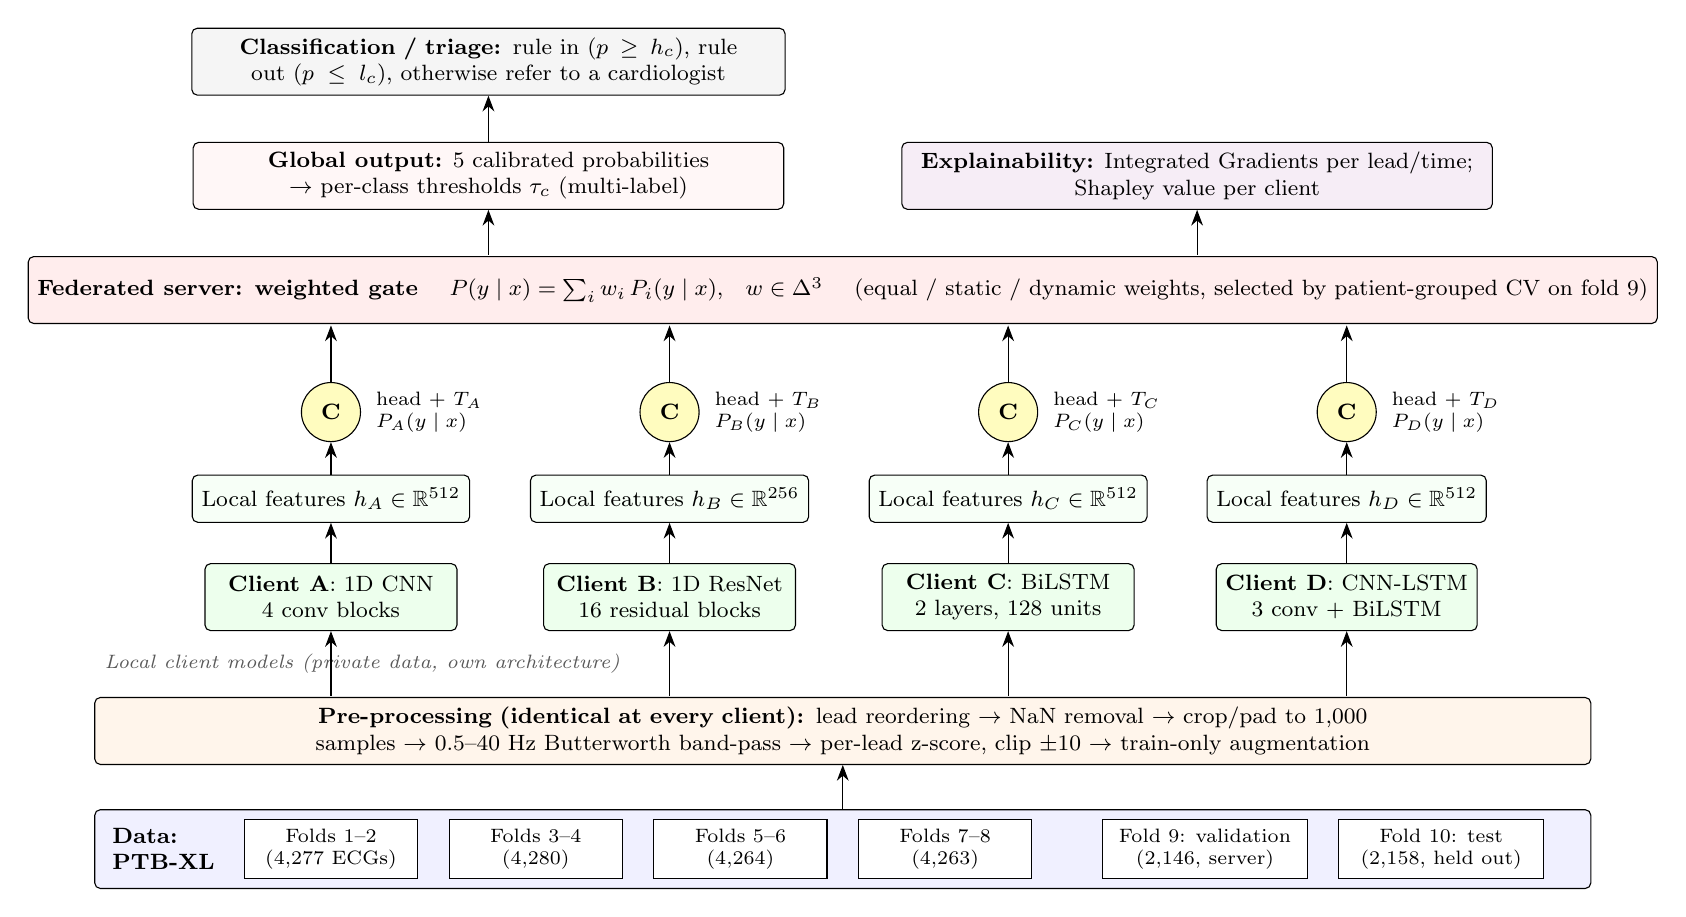
\begin{tikzpicture}[
  font=\footnotesize, >={Stealth[length=2mm]},
  box/.style={draw, rounded corners=2pt, align=center, minimum height=0.85cm, fill=#1},
  box/.default=white,
  lab/.style={font=\scriptsize\itshape, text=black!65}]
  % data (bottom)
  \node[box=blue!6, minimum width=19cm, minimum height=1.0cm] (data) at (0,0) {};
  \node[anchor=west, font=\footnotesize\bfseries, align=left] at (-9.4,0) {Data:\\PTB-XL};
  \node[draw, fill=white, minimum width=2.2cm, minimum height=0.65cm, align=center, font=\scriptsize] at (-6.5,0) {Folds 1--2\\(4,277 ECGs)};
  \node[draw, fill=white, minimum width=2.2cm, minimum height=0.65cm, align=center, font=\scriptsize] at (-3.9,0) {Folds 3--4\\(4,280)};
  \node[draw, fill=white, minimum width=2.2cm, minimum height=0.65cm, align=center, font=\scriptsize] at (-1.3,0) {Folds 5--6\\(4,264)};
  \node[draw, fill=white, minimum width=2.2cm, minimum height=0.65cm, align=center, font=\scriptsize] at (1.3,0) {Folds 7--8\\(4,263)};
  \node[draw, fill=white, minimum width=2.6cm, minimum height=0.65cm, align=center, font=\scriptsize] at (4.6,0) {Fold 9: validation\\(2,146, server)};
  \node[draw, fill=white, minimum width=2.6cm, minimum height=0.65cm, align=center, font=\scriptsize] at (7.6,0) {Fold 10: test\\(2,158, held out)};
  % preprocessing
  \node[box=orange!8, minimum width=19cm, text width=18.6cm] (prep) at (0,1.5)
    {\textbf{Pre-processing (identical at every client):} lead reordering $\rightarrow$ NaN removal $\rightarrow$
     crop/pad to 1,000 samples $\rightarrow$ 0.5--40 Hz Butterworth band-pass $\rightarrow$ per-lead z-score, clip $\pm10$
     $\rightarrow$ train-only augmentation};
  \draw[->] (data) -- (prep);
  \node[lab, anchor=west] at (-9.5,2.35) {Local client models (private data, own architecture)};
  % clients
  \foreach \x/\c/\a/\f in {-6.5/A/{1D CNN\\4 conv blocks}/{$h_A\in\mathbb{R}^{512}$},
                           -2.2/B/{1D ResNet\\16 residual blocks}/{$h_B\in\mathbb{R}^{256}$},
                            2.1/C/{BiLSTM\\2 layers, 128 units}/{$h_C\in\mathbb{R}^{512}$},
                            6.4/D/{CNN-LSTM\\3 conv + BiLSTM}/{$h_D\in\mathbb{R}^{512}$}} {
    \node[box=green!7, minimum width=3.2cm] (m\c) at (\x,3.2) {\textbf{Client \c}: \a};
    \node[box=green!3, minimum width=3.2cm, minimum height=0.6cm] (f\c) at (\x,4.45) {Local features \f};
    \node[draw, circle, fill=yellow!25, minimum size=0.75cm, font=\footnotesize\bfseries] (c\c) at (\x,5.55) {C};
    \node[anchor=west, font=\scriptsize, align=left] at (\x+0.45,5.55) {head + $T_\c$\\$P_\c(y\mid x)$};
    \draw[->] (\x,1.95) -- (m\c);
    \draw[->] (m\c) -- (f\c);
    \draw[->] (f\c) -- (c\c);
    \draw[->] (c\c) -- (\x,6.65);
  }
  % server
  \node[box=red!7, minimum width=19cm] (gate) at (0,7.1)
    {\textbf{Federated server: weighted gate} \quad $P(y\mid x)=\sum_{i} w_i\,P_i(y\mid x)$, \; $w\in\Delta^{3}$ \quad
     (equal / static / dynamic weights, selected by patient-grouped CV on fold 9)};
  \node[box=red!3, minimum width=7.5cm] (out) at (-4.5,8.55)
    {\textbf{Global output:} 5 calibrated probabilities\\$\rightarrow$ per-class thresholds $\tau_c$ (multi-label)};
  \node[box=violet!7, minimum width=7.5cm] (xai) at (4.5,8.55)
    {\textbf{Explainability:} Integrated Gradients per lead/time;\\Shapley value per client};
  \draw[->] (-4.5,7.55) -- (out);
  \draw[->] (4.5,7.55) -- (xai);
  \node[box=gray!8, minimum width=7.5cm, text width=7.3cm] (tri) at (-4.5,10.0)
    {\textbf{Classification / triage:} rule in ($p\ge h_c$), rule out ($p\le l_c$), otherwise refer to a cardiologist};
  \draw[->] (out) -- (tri);
\end{tikzpicture}}
\caption{Architecture of the proposed CardioSentinel model. Four clients hold disjoint, patient-separated
PTB-XL partitions, apply the same pre-processing, learn their own features with different network
architectures and expose only calibrated probabilities through their classifier heads (C). The
server combines the probabilities on the simplex, thresholds them per class and explains the global
output.}
\label{fig:arch}
\end{figure*}

\textit{Model progression.} The four clients were deliberately chosen to span the main families of
ECG networks, from purely convolutional to purely recurrent, so that their errors are as diverse as
possible. Client~A is a plain 1D CNN with four blocks of a 7-tap convolution (no bias), batch
normalisation, ReLU and max-pooling by two, with 32, 64, 128 and 256 channels. For an input
$x\in\mathbb{R}^{12\times 1000}$ each block computes
\begin{equation}
  h^{(l+1)} = \mathrm{MaxPool}_2\big(\mathrm{ReLU}(\mathrm{BN}(W^{(l)} * h^{(l)}))\big),
\end{equation}
and the final feature map is summarised by concatenated global average and global max pooling,
$\mathrm{AM}(h)=[\tfrac{1}{T}\sum_t h_t;\,\max_t h_t]$. Client~B is a 1D ResNet \cite{he2016resnet}
with a 7-tap, 64-channel stem and stages of 64, 128, 256 and 256 channels containing 3, 4, 6 and 3
residual blocks with 5-tap kernels, in which the last batch normalisation of each block is
initialised to zero so that each block starts as the identity, $h^{(l+1)}=\mathrm{ReLU}(F(h^{(l)})+S(h^{(l)}))$.
Client~C is a two-layer bidirectional LSTM \cite{hochreiter1997lstm,schuster1997bilstm} with 128
hidden units per direction that reads the 1,000 time steps directly; each direction updates
\begin{align}
  i_t &= \sigma(W_i x_t + U_i h_{t-1} + b_i), \nonumber\\
  f_t &= \sigma(W_f x_t + U_f h_{t-1} + b_f), \nonumber\\
  o_t &= \sigma(W_o x_t + U_o h_{t-1} + b_o), \nonumber\\
  g_t &= \tanh(W_c x_t + U_c h_{t-1} + b_c), \nonumber\\
  c_t &= f_t\odot c_{t-1} + i_t\odot g_t, \qquad h_t = o_t\odot\tanh(c_t),
\end{align}
and the forward and backward states are concatenated and pooled with $\mathrm{AM}(\cdot)$. Client~D is
a CNN-LSTM hybrid in which three convolutional blocks (32, 64 and 128 channels) shorten the sequence
from 1,000 to 125 steps before a one-layer BiLSTM with 128 hidden units, so that local wave
morphology is captured by the convolutions and rhythm context by the recurrence. All clients share
the same head, $\mathrm{Linear}(d\!\rightarrow\!256)\!\rightarrow\!\mathrm{ReLU}\!\rightarrow\!
\mathrm{Dropout}(0.3)\!\rightarrow\!\mathrm{Linear}(256\!\rightarrow\!5)$, and the same training
recipe, so that only the architecture and the data differ. On the held-out test fold this
progression moves the macro AUROC from 0.882--0.888 for the convolutional clients to 0.894 for the
BiLSTM and 0.896 for the CNN-LSTM, and the federated gate over all four reaches 0.905
(Section~\ref{sec:comparison}). An attention-based client was not part of the study.

Algorithm~\ref{alg:cardiomoe} summarises the complete method, from preprocessing to the explained,
triaged prediction.

\begin{algorithm}[!t]
\caption{CardioSentinel: one-shot federated classification of 12-lead ECGs}
\label{alg:cardiomoe}
\footnotesize
\begin{algorithmic}[1]
\Require Client partitions $\mathcal{D}_A,\dots,\mathcal{D}_D$ (folds 1--8), validation fold $\mathcal{V}$ (fold 9), test ECG $x$
\Ensure Calibrated probabilities $P(y\mid x)$, multi-label decision $y^{\mathrm{pred}}$, triage status, attributions
\For{each client $i\in\{A,B,C,D\}$ \textbf{in parallel}} \Comment{local, private}
  \State Pre-process every record of $\mathcal{D}_i$ (band-pass, z-score, clip)
  \State Train network $f_i$ with weighted BCE, AdamW and OneCycle; early-stop on macro AUROC of $\mathcal{V}$
  \State Fit temperature $T_i$ on $\mathcal{V}$; $P_i(y\mid x)\gets\sigma(f_i(x)/T_i)$
\EndFor
\State Server collects $P_i(y\mid v)$ for all $v\in\mathcal{V}$ \Comment{probabilities only}
\For{combiner $g\in(\text{equal},\text{static},\text{dynamic})$}
  \State Obtain out-of-fold predictions by patient-grouped 5-fold CV on $\mathcal{V}$; record macro AUROC $a_g$
\EndFor
\State $g^\star\gets$ equal; \textbf{for} $g$ in (static, dynamic): \textbf{if} $a_g\ge a_{g^\star}+0.002$ \textbf{then} $g^\star\gets g$
\State Refit $g^\star$ on $\mathcal{V}$; tune per-class thresholds $\tau_c$ and triage bands $(l_c,h_c)$ on its CV predictions
\State \textbf{Inference:} $P(y\mid x)\gets\sum_i w_i^{g^\star}(x)\,P_i(y\mid x)$; $y^{\mathrm{pred}}_c\gets[P(y_c\mid x)\ge\tau_c]$
\State Triage: rule in if $P(y_c\mid x)\ge h_c$, rule out if $\le l_c$, else refer
\State Explain $P(y_c\mid x)$ with Integrated Gradients over leads and time
\end{algorithmic}
\end{algorithm}

% ---------------------------------------------------------------------------------- B
\subsection{Preprocessing}
\label{sec:prep}

All preprocessing steps are listed in Table~\ref{tab:prep}. They are implemented once and executed
identically by every client, so no client-specific normalisation statistics are needed and no
information crosses client boundaries.

\textit{Label encoding and cleaning.} Each record's SCP-ECG statements are mapped to the
\texttt{diagnostic\_class} column of \texttt{scp\_statements.csv}, keeping only the 44 statements
flagged as diagnostic, and encoded as a multi-hot vector over (NORM, MI, STTC, CD, HYP). Records
without any diagnostic superclass cannot be labelled and are removed, which reduces the 21,799
records to 21,388. No other record is excluded.

\textit{Signal cleaning.} The 100-Hz waveforms are read with the WFDB library and reordered to I,
II, III, aVR, aVL, aVF, V1--V6, matching lead names case-insensitively. Non-finite samples are
replaced by zero, and every signal is cropped or zero-padded to exactly 1,000 samples. Baseline
wander and high-frequency noise are removed with a third-order Butterworth band-pass filter between
0.5 and 40~Hz applied forwards and backwards, so that the filter introduces no phase shift. The
filtered signals are stored in millivolts without normalisation.

\textit{Normalisation.} At load time each lead of each recording is z-scored with its own mean and
standard deviation, $x^{\mathrm{norm}}_{\ell t}=(x_{\ell t}-\mu_\ell)/\sigma_\ell$, clipped to $[-10,10]$, and a
lead whose standard deviation is below $10^{-6}$ is set to zero. Because the statistics are
per-recording, the normalisation needs no shared population statistics, which is essential in the
federated setting.

\textit{Augmentation and class balancing.} During training only, each signal is multiplied by a
random amplitude factor in $[0.9,1.1]$, white Gaussian noise is added at a signal-to-noise ratio
drawn from 20--30~dB, a sinusoidal baseline wander of 0.1--0.5~Hz with an amplitude of 0.05--0.3
standard deviations is added to every lead, and each lead is zeroed with probability 0.05. Class
imbalance is handled in the loss rather than by resampling: the positive term of each class is
weighted by the ratio of negatives to positives in the client's training data
(Section~\ref{sec:clf}). Modality alignment is not required because a single modality is used, but
all leads are aligned in time by construction.

\begin{table}[!t]
\centering
\caption{Pre-processing steps and parameters}
\label{tab:prep}
\footnotesize
\begin{tabular}{@{}p{2.1cm}p{5.9cm}@{}}
\toprule
Step & Method and parameters \\
\midrule
Label encoding & SCP codes $\rightarrow$ 5 diagnostic superclasses (44 diagnostic statements); multi-hot \\
Record cleaning & Remove records without a superclass (21,799 $\rightarrow$ 21,388) \\
Lead order & I, II, III, aVR, aVL, aVF, V1--V6 \\
Missing values & NaN/$\pm\infty$ $\rightarrow$ 0 \\
Length & 100 Hz, crop/zero-pad to 1,000 samples (10 s) \\
Filtering & Butterworth band-pass 0.5--40 Hz, order 3, zero-phase \\
Normalisation & Per-lead, per-record z-score; clip to $\pm10$; flat lead $\rightarrow$ 0 \\
Augmentation (train) & Amplitude $\times\mathcal{U}(0.9,1.1)$; noise SNR $\mathcal{U}(20,30)$ dB; wander 0.1--0.5 Hz, amp.\ $\mathcal{U}(0.05,0.3)$; lead dropout $p=0.05$ \\
Class balancing & BCE positive weight $=\#\text{neg}/\#\text{pos}$ per class \\
\bottomrule
\end{tabular}
\end{table}

% ---------------------------------------------------------------------------------- C
\subsection{Feature Analysis}
\label{sec:features}

No hand-crafted features are extracted. Every client learns its features end-to-end from the
normalised 12-lead signal, and the four architectures look at the signal in complementary ways, as
summarised in Table~\ref{tab:features}. The convolutional clients extract local morphological
features (QRS complexes, ST segments and T waves) whose receptive field grows with depth; the BiLSTM
integrates the whole 10-s recording in both directions and is sensitive to rhythm and to the
temporal relation between beats; the CNN-LSTM first compresses local morphology into 125 steps and
then models their sequence. All clients summarise the time axis with concatenated average and max
pooling, which preserves both the typical and the most extreme activation of each feature channel.

The correlation structure of the input explains why a lead-wise model is appropriate. The 12 leads
are not independent: the limb leads are linear combinations of two measured potentials, and
neighbouring precordial leads view the heart from similar angles. Fig.~\ref{fig:leadcorr} shows the
mean Pearson correlation between the normalised leads over 17,083 training recordings (one recording
with a flat lead was skipped). The leads facing the left ventricle form one strongly correlated group:
I, II, V4, V5 and V6 correlate with each other at $r=0.62$--$0.92$, and aVR mirrors them
($r=-0.69$ to $-0.90$). The inferior leads III and aVF form a second group ($r=0.74$), anti-correlated
with aVL ($r=-0.72$ for III), whereas the right precordial leads V1--V3 are only weakly related to the
lateral group (for example $r=0.02$ between V2 and V5). Much of the 12-lead input is therefore
redundant, while V1--V3 and the inferior leads carry largely separate information. Feature selection
is left to the networks, and lead dropout during training discourages them from relying on a single
lead.

Fusion is performed at the decision level. Feature-level fusion of the client embeddings
$h_i$ would require the clients to transmit internal representations of every patient and to agree
on a common embedding space, which both weakens privacy and is not meaningful for networks of
different design. Each client therefore maps its own features to calibrated class probabilities, and
only these are fused (Section~\ref{sec:fl}).

\begin{table}[!t]
\centering
\caption{Learned features per client}
\label{tab:features}
\footnotesize
\setlength{\tabcolsep}{3pt}
\resizebox{\columnwidth}{!}{%
\begin{tabular}{@{}llcl@{}}
\toprule
Client & Feature extractor & Pooled dim. & Main signal property \\
\midrule
A & 4 conv blocks, k=7, 32--256 ch. & 512 & Local wave morphology \\
B & ResNet, 16 blocks, k=5, 64--256 ch. & 512$\rightarrow$256 & Hierarchical morphology \\
C & 2-layer BiLSTM, 128 units, 1,000 steps & 512 & Rhythm, beat-to-beat context \\
D & 3 conv blocks + BiLSTM, 125 steps & 512 & Morphology and rhythm \\
\bottomrule
\end{tabular}}
\end{table}

\begin{figure}[!t]
\centering
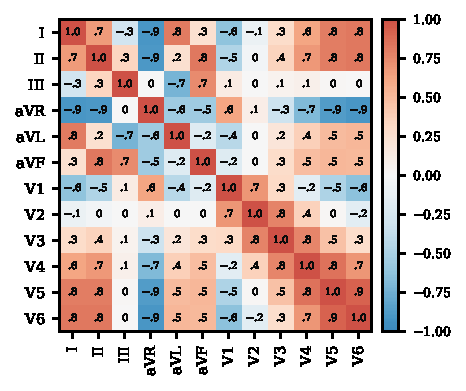
\includegraphics[width=0.85\columnwidth]{lead_corr}
\caption{Mean Pearson correlation between the 12 normalised leads over the training folds 1--8.}
\label{fig:leadcorr}
\end{figure}

% ---------------------------------------------------------------------------------- D
\subsection{Classification and Regression}
\label{sec:clf}

\textit{Classification.} The task is multi-label: a recording can belong to several superclasses at
once, and in PTB-XL 24.1\% of the retained records carry more than one superclass. The output layer
of each client therefore has five independent logits $z_{ic}$, and a sigmoid rather than a softmax
gives the class probabilities. Each client minimises the class-weighted binary cross-entropy
\begin{equation}
\begin{split}
\mathcal{L}_i = -\frac{1}{5N}\sum_{n=1}^{N}\sum_{c=1}^{5}\Big[&\beta_c\,y_{nc}\log\sigma(z_{nc})\\
 &+ (1-y_{nc})\log\big(1-\sigma(z_{nc})\big)\Big],
\end{split}
\end{equation}
with $\beta_c=N^{-}_c/N^{+}_c$ computed from the client's own training labels. After training, a
single temperature $T_i$ is fitted on the validation fold by minimising the same loss without
weights over $\sigma(z/T_i)$ \cite{guo2017calibration}, which rescales the confidence of the client
without changing its ranking. The final binary decision for class $c$ is
$y^{\mathrm{pred}}_c=[P(y_c\mid x)\ge\tau_c]$, where $\tau_c$ is the threshold that maximises the F1-score of
class $c$ on the validation predictions.

\textit{Regression.} The PTB-XL superclass task does not provide a continuous target such as a
severity score, so no regression head was trained and no regression metric (MAE, RMSE, $R^2$) is
reported. The only continuous quantities produced by the model are the calibrated probabilities,
which are used as graded risk scores by the triage rule: for each class a rule-in threshold $h_c$
and a rule-out threshold $l_c$ are fitted on validation data, findings with $l_c<P<h_c$ are referred
to a cardiologist, and coverage is always reported together with the precision and recall of the
automatically decided findings.

% ---------------------------------------------------------------------------------- E
\subsection{Federated Learning}
\label{sec:fl}

\textit{Clients and data split.} The $K=4$ clients receive the official PTB-XL training folds in
pairs: A folds 1--2, B folds 3--4, C folds 5--6 and D folds 7--8, i.e.\ about 4,270 records each. The
folds were constructed by the dataset authors so that all records of a patient lie in one fold and
the label distribution is similar across folds \cite{wagner2020ptbxl}; the partition is therefore
patient-disjoint and approximately IID with respect to the labels, and the heterogeneity of the
federation lies in the models: every client trains a different architecture with a different number
of parameters (0.44M to 6.73M). Fold 9 is held by the server as a validation set, and fold 10 is the
untouched test set.

\textit{Local training and communication.} Each client trains once, for up to 50 local epochs with
early stopping, and then fits its temperature. Federation therefore takes a single round: there is
no repeated exchange of parameters and no synchronisation between clients during training. At
fitting and inference time the server sends an ECG to the clients and receives one calibrated
5-dimensional probability vector from each, i.e.\ 20 numbers per ECG. In the experiments reported
here all parties were simulated on one machine, but no step of the method requires a client to
reveal its data, parameters or architecture. Fig.~\ref{fig:flow} shows the workflow and
Algorithm~\ref{alg:fl} the protocol.

\textit{Aggregation rule.} Parameter-averaging methods such as FedAvg \cite{mcmahan2017fedavg} update
a shared model as $\theta_{t+1}=\sum_{k=1}^{K}\frac{n_k}{n}\theta_k^{t+1}$, which is only defined
when all clients share the same parameter space. CardioSentinel instead aggregates the calibrated
predictions,
\begin{equation}
\label{eq:gate}
\begin{split}
P(y\mid x)&=\sum_{i=1}^{K} w_i(x)\,P_i(y\mid x),\\
w_i(x)&\ge 0,\qquad \sum_{i=1}^{K} w_i(x)=1,
\end{split}
\end{equation}
with the weights parameterised by a softmax so that the simplex constraint holds by construction.
This prediction-level aggregation is related to one-shot FL with ensembles of local models
\cite{guha2019oneshot} and to distillation-based schemes that also admit heterogeneous client models
\cite{li2019fedmd,lin2020feddf}; unlike the latter, it needs neither a public transfer dataset nor a
distillation step, because the calibrated mixture itself is the global model.
Three combiners of increasing complexity are considered. \emph{Equal weights} use $w_i=1/K$ and learn
nothing. \emph{Static weights} learn one global logit per client, $w=\mathrm{softmax}(\theta)$, by
minimising the binary cross-entropy of $P(y\mid x)$ on the validation data with full-batch Adam
(learning rate 0.05, 500 steps). The \emph{dynamic gate} is a per-patient mixture of experts
\cite{jacobs1991moe}: an MLP takes the 20 client probabilities and the four mean binary entropies
$H_i=-\frac{1}{5}\sum_c[p_{ic}\log p_{ic}+(1-p_{ic})\log(1-p_{ic})]$, passes them through a 32-unit
ReLU layer with dropout 0.2 and outputs $w(x)=\mathrm{softmax}(\cdot)$; its last layer is
initialised to zero so that it starts from equal weights, and it is trained with AdamW and early
stopping on a patient-grouped 20\% inner hold-out. All three are evaluated by patient-grouped
five-fold cross-validation inside the validation fold, and the selection rule of
Algorithm~\ref{alg:cardiomoe} adopts a more complex combiner only if its cross-validated macro AUROC
exceeds that of the current choice by at least 0.002. This rule was fixed before the multi-seed test
evaluation.

\textit{Privacy benefit.} Raw ECGs, patient identifiers, model parameters, gradients and internal
embeddings never leave a client. The server observes only five calibrated probabilities per client
and ECG, which is the information a clinical decision-support service would return anyway. The
scheme does not by itself provide formal guarantees such as differential privacy, and the server
must hold a labelled validation set to fit the gate.

\begin{figure}[!t]
\centering
\resizebox{\columnwidth}{!}{%
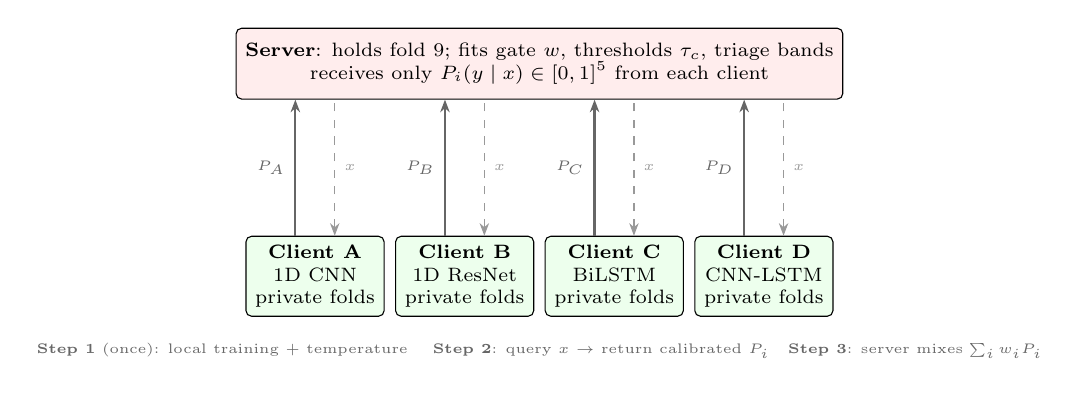
\begin{tikzpicture}[font=\scriptsize, >={Stealth[length=1.6mm]},
  cl/.style={draw, rounded corners=2pt, fill=green!7, minimum width=1.5cm, minimum height=1.0cm, align=center},
  sv/.style={draw, rounded corners=2pt, fill=red!7, minimum width=7.6cm, minimum height=0.9cm, align=center}]
  \node[sv] (srv) at (0,2.7) {\textbf{Server}: holds fold 9; fits gate $w$, thresholds $\tau_c$, triage bands\\
    receives only $P_i(y\mid x)\in[0,1]^5$ from each client};
  \foreach \x/\c/\a in {-2.85/A/1D CNN, -0.95/B/1D ResNet, 0.95/C/BiLSTM, 2.85/D/CNN-LSTM} {
    \node[cl] (k\c) at (\x,0) {\textbf{Client \c}\\\a\\private folds};
    \draw[->, thick, black!60] ($(k\c.north)+(-0.25,0)$) -- node[left, font=\tiny, align=right]{$P_\c$} ($(srv.south -| k\c.north)+(-0.25,0)$);
    \draw[<-, black!40, dashed] ($(k\c.north)+(0.25,0)$) -- node[right, font=\tiny]{$x$} ($(srv.south -| k\c.north)+(0.25,0)$);
  }
  \node[font=\tiny, align=center, text=black!60] at (0,-0.95)
    {\textbf{Step 1} (once): local training + temperature \quad \textbf{Step 2}: query $x$ $\rightarrow$ return calibrated $P_i$\quad
     \textbf{Step 3}: server mixes $\sum_i w_iP_i$};
\end{tikzpicture}}
\caption{Federated workflow. Clients train once on private data; afterwards the server sends an ECG
$x$ (dashed) and receives calibrated probabilities (solid). No parameters or raw training data are
exchanged.}
\label{fig:flow}
\end{figure}

\begin{algorithm}[!t]
\caption{One-shot federated protocol and gate selection}
\label{alg:fl}
\footnotesize
\begin{algorithmic}[1]
\Require $K=4$ clients with private data $\mathcal{D}_i$; server validation set $\mathcal{V}$ with patient IDs
\State \textbf{Round 1 (only round):} each client trains $f_i$ on $\mathcal{D}_i$, fits $T_i$, exposes $P_i(y\mid x)=\sigma(f_i(x)/T_i)$
\State Server queries all clients on $\mathcal{V}$: $\mathbf{P}\in[0,1]^{|\mathcal{V}|\times K\times 5}$
\State Split $\mathcal{V}$ into 5 patient-grouped folds
\For{combiner $g$ and CV fold $j$}
  \State Fit $g$ on the other 4 folds by minimising BCE of $\sum_i w_i P_i$; predict fold $j$
\EndFor
\State Select $g^\star$ by the $\ge0.002$ macro-AUROC rule; refit on all of $\mathcal{V}$
\State \textbf{Deployment:} for a new ECG, query clients and return $\sum_i w_i^{g^\star}P_i$
\end{algorithmic}
\end{algorithm}

% ---------------------------------------------------------------------------------- F
\subsection{Explainable AI}
\label{sec:xai-method}

Two complementary explanations are produced for the global model, one at the level of the input
signal and one at the level of the federation.

\textit{Signal-level attributions.} Because the global output of Eq.~(\ref{eq:gate}) with equal
weights is a differentiable function of the input, $F_c(x)=\frac{1}{K}\sum_i\sigma(z_{ic}(x)/T_i)$,
it can be explained with Integrated Gradients (IG) \cite{sundararajan2017ig}. For class $c$ and a
baseline $x'$, the attribution of input sample $(\ell,t)$ is
\begin{equation}
\mathrm{IG}_{\ell t}(x)=(x_{\ell t}-x'_{\ell t})\int_{0}^{1}\frac{\partial F_c\big(x'+\alpha(x-x')\big)}{\partial x_{\ell t}}\,d\alpha,
\end{equation}
approximated with a 32-step Riemann sum. The baseline is the all-zero signal, which after per-lead
z-scoring corresponds to every lead resting at its own mean. IG satisfies completeness, i.e.\ the
attributions sum to $F_c(x)-F_c(x')$, and is computed on the whole gate rather than on a single
client. Global lead importance for class $c$ is the share of $\sum_t|\mathrm{IG}_{\ell t}|$ falling on
each lead, averaged over the positive validation records of that class; local explanations show
$|\mathrm{IG}_{\ell t}|$ along time for the leads with the largest share. The faithfulness of the
attributions is checked with a deletion test: the $k$ leads with the largest attribution are set to
zero and the drop in $F_c$ is compared with that obtained when $k$ random leads are removed. Gradient
methods were preferred over Grad-CAM \cite{selvaraju2017gradcam} because two of the four clients have
no convolutional feature map at the output, and over sampling-based SHAP \cite{lundberg2017shap}
because of the 12{,}000-dimensional input.

\textit{Federation-level attributions.} The contribution of each institution to the global macro
AUROC $v(S)$ of an equal-weight sub-federation $S\subseteq\{A,B,C,D\}$ is quantified with the Shapley
value \cite{shapley1953},
\begin{equation}
\phi_i=\sum_{S\subseteq\mathcal{K}\setminus\{i\}}\frac{|S|!\,(K-|S|-1)!}{K!}\big[v(S\cup\{i\})-v(S)\big],
\end{equation}
with $v(\emptyset)=0.5$, the AUROC of an uninformative ranking. The 15 non-empty subsets are evaluated
exactly, so no sampling approximation is needed. All explanations are computed on validation (fold 9)
records or on subset results that were already part of the evaluation; the test fold is not used to
generate them.

\section{Results and Analysis}
\label{sec:results}

% ---------------------------------------------------------------------------------- A
\subsection{Dataset Description}
\label{sec:dataset}

All experiments use PTB-XL v1.0.3 \cite{wagner2020ptbxl}, an open-access (CC BY 4.0) collection
distributed through PhysioNet \cite{goldberger2000}. It contains 21,799 clinical 12-lead ECGs of
10~s from 18,869 patients, recorded with Schiller devices and annotated with SCP-ECG statements by
up to two cardiologists; the 100-Hz version of the waveforms is used here. As described in
Section~\ref{sec:prep}, 411 records without a diagnostic superclass were removed, leaving 21,388
records from 18,617 patients. The mean age of the retained patients is 59.4 $\pm$ 16.8 years
(ages above 89 are stored as a placeholder in PTB-XL and were excluded from this mean), and 48.1\%
of the records belong to female patients. The labels are the five diagnostic superclasses: normal
ECG (NORM), myocardial infarction (MI), ST/T change (STTC), conduction disturbance (CD) and
hypertrophy (HYP). Because a recording may carry several superclasses, the mean number of labels per
record is 1.30 and 24.1\% of the records are multi-label.

The official stratified folds of PTB-XL were used without modification, which guarantees that all
recordings of a patient lie in a single fold. Folds 1--8 (17,084 records, 80\%) form the training
data and are divided among the four clients, fold 9 (2,146 records, 10\%) is the validation set
used for early stopping, calibration, thresholds and the gate, and fold 10 (2,158 records from
1,877 patients, 10\%) is the test set. The split is therefore 80/10/10 rather than 80/20: the
separate validation fold prevents any model or gate choice from being tuned on the test data.
Table~\ref{tab:dataset} lists the records, patients and class counts of every partition, and
Fig.~\ref{fig:classdist} shows the class distribution. NORM is the most frequent superclass
(44.5\% of records) and HYP the rarest (12.4\%), and the class proportions of the four clients
differ by less than one percentage point.

\begin{table*}[!t]
\centering
\caption{Dataset details: records, patients and positive labels per partition (prevalence in \% in parentheses)}
\label{tab:dataset}
\footnotesize
\begin{tabular}{@{}lcccccccc@{}}
\toprule
Partition & Folds & Records & Patients & NORM & MI & STTC & CD & HYP \\
\midrule
Client A & 1, 2 & 4{,}277 & 3{,}676 & 1{,}907 & 1{,}087 & 1{,}050 & 966 & 527 \\
Client B & 3, 4 & 4{,}280 & 3{,}722 & 1{,}918 & 1{,}079 & 1{,}042 & 981 & 525 \\
Client C & 5, 6 & 4{,}264 & 3{,}725 & 1{,}869 & 1{,}125 & 1{,}060 & 990 & 535 \\
Client D & 7, 8 & 4{,}263 & 3{,}700 & 1{,}902 & 1{,}088 & 1{,}034 & 970 & 532 \\
\midrule
Train & 1--8 & 17{,}084 & 14{,}823 & 7{,}596 (44.5) & 4{,}379 (25.6) & 4{,}186 (24.5) & 3{,}907 (22.9) & 2{,}119 (12.4) \\
Validation & 9 & 2{,}146 & 1{,}917 & 955 (44.5) & 540 (25.2) & 528 (24.6) & 495 (23.1) & 268 (12.5) \\
Test & 10 & 2{,}158 & 1{,}877 & 963 (44.6) & 550 (25.5) & 521 (24.1) & 496 (23.0) & 262 (12.1) \\
\midrule
Total & 1--10 & 21{,}388 & 18{,}617 & 9{,}514 (44.5) & 5{,}469 (25.6) & 5{,}235 (24.5) & 4{,}898 (22.9) & 2{,}649 (12.4) \\
\bottomrule
\end{tabular}

\end{table*}

\begin{figure}[!t]
\centering
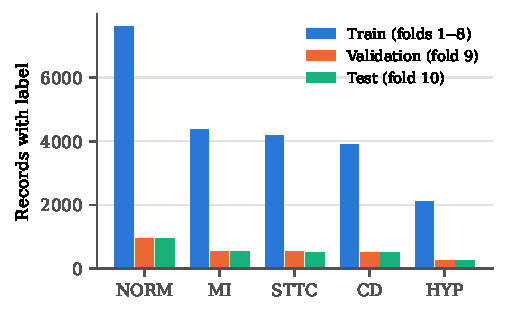
\includegraphics[width=\columnwidth]{class_distribution}
\caption{Number of records carrying each diagnostic superclass in the training, validation and test
folds (multi-label, so a record can be counted in several classes).}
\label{fig:classdist}
\end{figure}

% ---------------------------------------------------------------------------------- B
\subsection{Experimental Setup}
\label{sec:setup}

All networks were implemented in PyTorch \cite{paszke2019pytorch} and trained on an Apple M1
MacBook Air with 8~GB of unified memory using the Metal (MPS) backend, under macOS, Python 3.11.17 and PyTorch 2.14.1. Mixed precision was not
used. A mean training epoch took 26.8~s for Client~A, 38.5~s for Client~B, 65.4~s for Client~C and
28.2~s for Client~D. Every experiment was repeated with the random seeds 42, 43 and 44, and results
are reported as mean $\pm$ standard deviation over the three seeds. Table~\ref{tab:hyper} lists all
hyperparameters; they are identical for every client so that only the architecture and the data
differ.

\begin{table}[!t]
\centering
\caption{Hyperparameters}
\label{tab:hyper}
\footnotesize
\begin{tabular}{@{}p{3.3cm}p{4.7cm}@{}}
\toprule
Parameter & Value \\
\midrule
Input & $12\times1000$ (10 s at 100 Hz) \\
Number of clients & 4 (A, B, C, D), 2 PTB-XL folds each \\
Communication rounds & 1 (one-shot; probabilities only) \\
Local epochs & up to 50; early stopping, patience 8 \\
Early-stopping criterion & macro AUROC on fold 9 \\
Batch size & 128 \\
Optimizer & AdamW \cite{loshchilov2019adamw}, weight decay $10^{-2}$ \\
Learning rate & $10^{-3}$, OneCycle schedule \cite{smith2019superconvergence} \\
Loss & BCE with logits, positive weight $N^-_c/N^+_c$ \\
Gradient clipping & global norm 1.0 \\
Head & Linear 256, ReLU, dropout 0.3, Linear 5 \\
Activation & ReLU (BiLSTM: sigmoid/tanh gates) \\
Calibration & 1 temperature per client, LBFGS on fold 9 \\
Aggregation & equal / static / dynamic gate; selection by 5-fold patient-grouped CV, margin 0.002 \\
Static gate & 4 weights, Adam lr 0.05, 500 steps \\
Dynamic gate & MLP 24--32--4, dropout 0.2, AdamW lr $10^{-3}$, $\le$300 epochs, patience 30 \\
Thresholds & per class, max.\ F1 on fold 9 \\
Bootstrap & 1,000 resamples (95\% CI, paired) \\
Seeds & 42, 43, 44 \\
\bottomrule
\end{tabular}
\end{table}

Because the task is multi-label, every metric is first computed per class from that class's
confusion counts $TP_c$, $FP_c$, $FN_c$ and $TN_c$ on the $N$ test records, and then macro-averaged
over the five classes:
\begin{align}
\mathrm{Precision}_c &= \frac{TP_c}{TP_c+FP_c},\qquad \mathrm{Recall}_c = \frac{TP_c}{TP_c+FN_c},\\
\mathrm{Specificity}_c &= \frac{TN_c}{TN_c+FP_c},\\
\mathrm{F1}_c &= \frac{2\,\mathrm{Precision}_c\,\mathrm{Recall}_c}{\mathrm{Precision}_c+\mathrm{Recall}_c},\\
\mathrm{Acc}_{\text{label}} &= \frac{1}{5}\sum_{c=1}^{5}\frac{TP_c+TN_c}{N},\\
\mathrm{Acc}_{\text{exact}} &= \frac{1}{N}\sum_{n=1}^{N}\big[\mathbf y^{\mathrm{pred}}_n=\mathbf y_n\big].
\end{align}
Label-wise accuracy (reported as ``Acc.'') counts every one of the five decisions per record, whereas
exact-match accuracy requires all five decisions of a record to be correct. The area under the ROC
curve is $\mathrm{AUROC}_c=\int_0^1\mathrm{TPR}_c\,d\,\mathrm{FPR}_c$, the probability that a random
positive is ranked above a random negative, and is threshold-free; AUPRC is the area under the
precision--recall curve. Macro AUROC is the primary metric, because it is insensitive to the
decision thresholds and to class prevalence, and its 95\% confidence interval is obtained with 1,000
bootstrap resamples of the test records \cite{efron1993bootstrap}. Differences between two models are
assessed with a paired bootstrap on the same resamples. Regression metrics (MAE, RMSE, $R^2$) do not
apply because the task has no continuous target (Section~\ref{sec:clf}).

% ---------------------------------------------------------------------------------- C
\subsection{Comparison of Performance Metrics With Traditional Machine Learning Models and Unimodal Models}
\label{sec:comparison}

Table~\ref{tab:main} compares the proposed model with the individual deep clients, with the two
learned aggregation variants and with a centrally trained reference. All rows were evaluated once
on the same test fold with thresholds chosen on fold 9. The traditional classifiers use 172
hand-crafted features computed from the filtered, un-normalised signal: per-lead amplitude statistics
(standard deviation, minimum, maximum, range, skewness, kurtosis, mean absolute slope), relative
spectral power in the 0.5--5, 5--15 and 15--40~Hz bands, heart rate and RR-interval variability from
R peaks detected in lead II, and per-lead median R, S, ST and T amplitudes around those peaks. They
were trained on the pooled folds 1--8, Platt-scaled on fold 9 and thresholded on fold 9 like the deep
models; Random Forest and XGBoost were run with the three seeds, while logistic regression, the RBF SVM
and KNN are deterministic.

\begin{table*}[!t]
\centering
\caption{Comparison with traditional machine-learning models, the individual deep clients and the
aggregation variants on the PTB-XL test fold (mean $\pm$ SD over 3 seeds; Acc.\ = label-wise
accuracy; Prec., Rec., F1, AUROC and AUPRC are macro averages over the five superclasses)}
\label{tab:main}
\footnotesize
\begin{tabular}{@{}llcccccc@{}}
\toprule
Model & Params & Acc. (\%) & Prec. (\%) & Rec. (\%) & F1 (\%) & AUROC & AUPRC \\
\midrule
\multicolumn{8}{@{}l}{\emph{Traditional machine learning (172 hand-crafted features, pooled folds 1--8)}}\\
Logistic Regression & -- & 84.4 $\pm$ 0.0 & 65.3 $\pm$ 0.0 & 71.7 $\pm$ 0.0 & 68.2 $\pm$ 0.0 & 0.880 $\pm$ 0.000 & 0.724 $\pm$ 0.000 \\
SVM (RBF) & -- & 85.8 $\pm$ 0.0 & 67.3 $\pm$ 0.0 & 74.5 $\pm$ 0.0 & 70.6 $\pm$ 0.0 & 0.898 $\pm$ 0.000 & 0.772 $\pm$ 0.000 \\
Random Forest & -- & 86.2 $\pm$ 0.2 & 69.1 $\pm$ 0.8 & 74.0 $\pm$ 1.2 & 71.2 $\pm$ 0.2 & 0.902 $\pm$ 0.001 & 0.778 $\pm$ 0.001 \\
KNN & -- & 82.2 $\pm$ 0.0 & 60.8 $\pm$ 0.0 & 68.9 $\pm$ 0.0 & 64.4 $\pm$ 0.0 & 0.859 $\pm$ 0.000 & 0.700 $\pm$ 0.000 \\
XGBoost & -- & 86.8 $\pm$ 0.0 & 69.7 $\pm$ 0.2 & 76.3 $\pm$ 0.5 & 72.6 $\pm$ 0.2 & 0.909 $\pm$ 0.002 & 0.789 $\pm$ 0.003 \\
\midrule
\multicolumn{8}{@{}l}{\emph{Single deep clients (25\% of training data each)}}\\
Client A: 1D CNN & 0.44M & 84.8 $\pm$ 0.2 & 64.6 $\pm$ 0.6 & 72.6 $\pm$ 0.8 & 68.0 $\pm$ 0.3 & 0.888 $\pm$ 0.002 & 0.738 $\pm$ 0.005 \\
Client B: 1D ResNet & 6.73M & 84.0 $\pm$ 0.8 & 63.0 $\pm$ 1.3 & 73.4 $\pm$ 1.8 & 67.2 $\pm$ 0.4 & 0.882 $\pm$ 0.002 & 0.721 $\pm$ 0.005 \\
Client C: BiLSTM & 0.67M & 85.5 $\pm$ 0.3 & 66.2 $\pm$ 1.2 & 73.3 $\pm$ 0.5 & 69.2 $\pm$ 0.3 & 0.894 $\pm$ 0.000 & 0.745 $\pm$ 0.003 \\
Client D: CNN-LSTM & 0.47M & 85.7 $\pm$ 0.8 & 67.0 $\pm$ 2.8 & 72.2 $\pm$ 3.1 & 69.0 $\pm$ 0.1 & 0.896 $\pm$ 0.001 & 0.749 $\pm$ 0.006 \\
\midrule
\multicolumn{8}{@{}l}{\emph{Aggregation of the four clients}}\\
Static learned weights & 4 & 86.6 $\pm$ 0.3 & 68.5 $\pm$ 0.9 & 72.8 $\pm$ 0.8 & 70.3 $\pm$ 0.3 & 0.903 $\pm$ 0.001 & 0.764 $\pm$ 0.004 \\
Dynamic gate & $\approx$1k & 86.4 $\pm$ 0.3 & 68.1 $\pm$ 1.2 & 72.9 $\pm$ 1.3 & 70.2 $\pm$ 0.1 & 0.901 $\pm$ 0.001 & 0.759 $\pm$ 0.002 \\
\textbf{Proposed (equal-weight gate)} & 8.31M & 86.9 $\pm$ 0.2 & 69.8 $\pm$ 0.9 & 72.5 $\pm$ 2.1 & 70.7 $\pm$ 0.6 & 0.905 $\pm$ 0.000 & 0.767 $\pm$ 0.002 \\
\midrule
\multicolumn{8}{@{}l}{\emph{Centralised reference (data pooled, not federated)}}\\
CNN-LSTM on folds 1--8 & 0.47M & 86.4 $\pm$ 0.7 & 68.5 $\pm$ 1.2 & 74.0 $\pm$ 0.6 & 70.7 $\pm$ 0.8 & 0.909 $\pm$ 0.001 & 0.774 $\pm$ 0.002 \\
\bottomrule
\end{tabular}

\end{table*}

The four deep clients, each trained on only a quarter of the training data, reach test macro AUROCs
between 0.882 (Client B, 1D ResNet) and 0.896 (Client D, CNN-LSTM). The recurrent clients rank best:
the BiLSTM (0.894) and the CNN-LSTM (0.896) outperform both convolutional clients, and the ResNet,
despite having the most parameters (6.73M), is the weakest, which is consistent with its early
stopping after 13.7 epochs on average (Table~\ref{tab:clienttrain}) and indicates over-fitting on
4,280 records. The proposed equal-weight gate raises the macro AUROC to 0.905 $\pm$ 0.000, the
label-wise accuracy to 86.9\% (from at most 85.7\%), the macro F1 to 70.7\% (from at most 69.2\%)
and the macro precision to 69.8\% (from at most 67.0\%), while keeping the recall (72.5\%) at the
level of the clients. Its AUPRC of 0.767 is also the highest among the federated models. A CNN-LSTM
trained centrally on all eight training folds, which is not possible when the data cannot be pooled,
attains 0.909 $\pm$ 0.001 macro AUROC and the same macro F1 of 70.7\%; the federated gate therefore
recovers about 70\% of the AUROC lost by splitting the data (0.896 $\rightarrow$ 0.905 of the
0.896 $\rightarrow$ 0.909 gap) and is tied with the pooled model in F1. As an external reference for
feature-based learning on the same test fold, the wavelet-feature neural network of
\cite{strodthoff2021} reported a superdiagnostic macro AUROC of 0.874.

The traditional classifiers turn out to be strong baselines. Trained on all pooled data, XGBoost
reaches a macro AUROC of 0.909 $\pm$ 0.002 and a macro F1 of 72.6\%, and Random Forest 0.902 and
71.2\%, so the best of them matches the pooled CNN-LSTM in AUROC and exceeds both it and the
federated gate in F1; KNN (0.859) and logistic regression (0.880) are clearly weaker. The amplitude
features are the likely reason: they keep the absolute voltages that the per-recording z-scoring of
the deep models removes, and these voltages define hypertrophy. The comparison is, however, not a
federated one, because these models see four times as much data as each client. Table~\ref{tab:tradlocal}
therefore trains the same classifiers on a single client's two folds. Under this restriction XGBoost
reaches 0.898 on average and Random Forest 0.893--0.895, i.e.\ the level of the best deep clients
(0.894--0.896), and every locally trained model, traditional or deep, remains below the federated
gate (0.905).

\begin{table}[!t]
\centering
\caption{Traditional classifiers trained locally (one client's folds; mean $\pm$ SD over clients A--D,
seed 42) or on pooled data (mean $\pm$ SD over 3 seeds), compared with the best deep clients (test fold)}
\label{tab:tradlocal}
\footnotesize
\setlength{\tabcolsep}{3pt}
\resizebox{\columnwidth}{!}{\begin{tabular}{@{}lcccc@{}}
\toprule
 & \multicolumn{2}{c}{Local (one client, mean of A--D)} & \multicolumn{2}{c}{Pooled (folds 1--8)} \\
\cmidrule(lr){2-3}\cmidrule(l){4-5}
Model & AUROC & F1 (\%) & AUROC & F1 (\%) \\
\midrule
Logistic Regression & 0.870 $\pm$ 0.001 & 67.0 $\pm$ 0.1 & 0.880 $\pm$ 0.000 & 68.2 $\pm$ 0.0 \\
SVM (RBF) & 0.886 $\pm$ 0.002 & 68.8 $\pm$ 0.3 & 0.898 $\pm$ 0.000 & 70.6 $\pm$ 0.0 \\
Random Forest & 0.894 $\pm$ 0.001 & 69.8 $\pm$ 0.2 & 0.902 $\pm$ 0.001 & 71.2 $\pm$ 0.2 \\
KNN & 0.847 $\pm$ 0.004 & 63.3 $\pm$ 0.6 & 0.859 $\pm$ 0.000 & 64.4 $\pm$ 0.0 \\
XGBoost & 0.898 $\pm$ 0.002 & 70.4 $\pm$ 0.4 & 0.909 $\pm$ 0.002 & 72.6 $\pm$ 0.2 \\
\midrule
Deep client C (BiLSTM) & 0.894 $\pm$ 0.000 & 69.2 $\pm$ 0.3 & -- & -- \\
Deep client D (CNN-LSTM) & 0.896 $\pm$ 0.001 & 69.0 $\pm$ 0.1 & -- & -- \\
\bottomrule
\end{tabular}
}
\end{table}

The study uses a single input modality, the 12-lead ECG, so a comparison of unimodal and multimodal
models in the strict sense is not possible. Table~\ref{tab:clientgate} instead contrasts each
single-architecture client with the federated combination of all four, per superclass. The gate
achieves the highest AUROC in every class, and its largest gain over the best client is observed for
the hardest class, HYP (0.828 versus at most 0.809). This indicates that the clients make partly
independent errors that the combination averages out, the same mechanism that motivates
multimodal fusion, but obtained here from architectural rather than modal diversity.

\begin{table}[!t]
\centering
\caption{Single clients versus the federated gate: test AUROC per superclass (mean of 3 seeds; best in bold)}
\label{tab:clientgate}
\footnotesize
\setlength{\tabcolsep}{3.5pt}
\begin{tabular}{@{}lccccc|c@{}}
\toprule
Model & NORM & MI & STTC & CD & HYP & Macro \\
\midrule
Client A (1D CNN) & 0.926 & 0.891 & 0.925 & 0.900 & 0.798 & 0.888 \\
Client B (1D ResNet) & 0.922 & 0.877 & 0.918 & 0.884 & 0.808 & 0.882 \\
Client C (BiLSTM) & 0.931 & 0.901 & 0.926 & 0.902 & 0.809 & 0.894 \\
Client D (CNN-LSTM) & 0.933 & 0.906 & 0.923 & 0.909 & 0.808 & 0.896 \\
\textbf{Proposed} & \textbf{0.938} & \textbf{0.912} & \textbf{0.933} & \textbf{0.914} & \textbf{0.828} & 0.905 \\
\bottomrule
\end{tabular}

\end{table}

The gain over the best single client is statistically significant. In a paired bootstrap on the test
fold, the macro AUROC of the gate exceeds that of the best client chosen on fold 9 by +0.012
[+0.009, +0.016] for seed 42 (Client C), +0.011 [+0.007, +0.014] for seed 43 (Client C) and +0.009
[+0.005, +0.013] for seed 44 (Client D), so every confidence interval lies above zero. The macro F1
improves by +0.018 [+0.009, +0.028], +0.010 [$-$0.001, +0.021] and +0.024 [+0.014, +0.034],
respectively, with the interval excluding zero in two of the three seeds. Fig.~\ref{fig:modelcomp}
summarises the macro AUROC of all models.

\begin{figure}[!t]
\centering
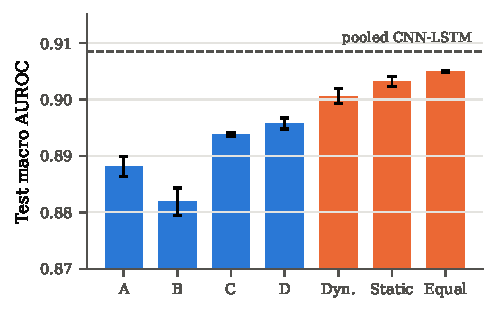
\includegraphics[width=\columnwidth]{model_comparison}
\caption{Test macro AUROC of the four clients and the three aggregation variants (mean $\pm$ SD over
3 seeds). The dashed line marks the centrally trained CNN-LSTM.}
\label{fig:modelcomp}
\end{figure}

% ---------------------------------------------------------------------------------- D
\subsection{Ablation Experiments}
\label{sec:ablation}

\subsubsection{Modality Ablation Experiment}
Since the ECG is the only modality, the input-source ablation was carried out over the
participating institutions: every one of the 15 non-empty subsets of $\{A,B,C,D\}$ was combined with
equal weights and evaluated on fold 9 (cross-validated) and on the test fold. The results, ordered by
the number of clients, are given in Table~\ref{tab:subsets}, and Table~\ref{tab:shapley} converts them
into a Shapley value per client.
\begin{table}[!t]
\centering
\caption{Client-subset ablation (equal-weight gate; mean over 3 seeds, test SD shown)}
\label{tab:subsets}
\footnotesize
\setlength{\tabcolsep}{4pt}
\begin{tabular}{@{}clccc@{}}
\toprule
\#Clients & Subset & Fold-9 CV AUROC & Test AUROC & $\Delta$ vs.\ ABCD \\
\midrule
4 & \textbf{ABCD} & 0.909 & 0.905 $\pm$ 0.000 & 0.000 \\
\midrule
3 & ACD & 0.908 & 0.905 $\pm$ 0.000 & 0.000 \\
3 & BCD & 0.908 & 0.904 $\pm$ 0.001 & -0.001 \\
3 & ABC & 0.906 & 0.901 $\pm$ 0.000 & -0.004 \\
3 & ABD & 0.905 & 0.902 $\pm$ 0.001 & -0.003 \\
\midrule
2 & CD & 0.907 & 0.903 $\pm$ 0.001 & -0.002 \\
2 & AC & 0.905 & 0.900 $\pm$ 0.000 & -0.005 \\
2 & AD & 0.904 & 0.901 $\pm$ 0.001 & -0.004 \\
2 & BC & 0.903 & 0.898 $\pm$ 0.001 & -0.007 \\
2 & BD & 0.903 & 0.900 $\pm$ 0.001 & -0.005 \\
2 & AB & 0.899 & 0.895 $\pm$ 0.001 & -0.010 \\
\midrule
1 & C & 0.900 & 0.894 $\pm$ 0.000 & -0.011 \\
1 & D & 0.898 & 0.896 $\pm$ 0.001 & -0.009 \\
1 & A & 0.893 & 0.888 $\pm$ 0.002 & -0.017 \\
1 & B & 0.886 & 0.882 $\pm$ 0.003 & -0.023 \\
\bottomrule
\end{tabular}

\end{table}

The full federation ABCD is the best configuration on both splits (fold 9: 0.909; test: 0.905).
Every two-client combination outperforms every single client on the test fold, so most of the gain
comes from combining heterogeneous models at all, and adding clients yields diminishing returns
(single: at most 0.896; pairs: at most 0.903; triples: at most 0.905). Removing the recurrent clients
hurts most: dropping D lowers the test AUROC by 0.004 and dropping C by 0.003, whereas dropping A or B
costs at most 0.001. The Shapley values in Table~\ref{tab:shapley} confirm this ranking (C and D
largest, B smallest), but they also show that the four contributions are of the same order
(0.097--0.105 on the test fold). This explains why equal weighting works well: the learned static
weights assign almost nothing to Client A (0.001 on average), although its marginal contribution to
the federation is comparable to that of the other clients.

\begin{table}[!t]
\centering
\caption{Shapley value $\phi_i$ of each client for the macro AUROC of the equal-weight federation
($v(\emptyset)=0.5$) and the mean learned static weight}
\label{tab:shapley}
\footnotesize
\setlength{\tabcolsep}{4pt}
\begin{tabular}{@{}lcccc@{}}
\toprule
Client & Architecture & $\phi$ (fold 9) & $\phi$ (test) & Static weight $w_i$ \\
\midrule
A & 1D CNN & 0.1009 & 0.0998 & 0.001 \\
B & 1D ResNet & 0.0980 & 0.0971 & 0.042 \\
C & BiLSTM & 0.1055 & 0.1033 & 0.549 \\
D & CNN-LSTM & 0.1043 & 0.1047 & 0.407 \\
\midrule
Sum & -- & 0.4087 & 0.4050 & 1.000 \\
\bottomrule
\end{tabular}

\end{table}

\subsubsection{Feature Fusion Module Ablation Experiments}
Table~\ref{tab:fusion} compares the three fusion strategies of Section~\ref{sec:fl}: equal weights,
learned static weights and the dynamic per-patient gate. All three are late (decision-level) fusion
strategies, because the clients do not share embeddings; early or feature-level fusion is excluded by
the privacy constraint. The validation columns are the patient-grouped cross-validated values used for
selection, and the test columns were obtained afterwards.

\begin{table*}[!t]
\centering
\caption{Ablation of the fusion strategy (fold-9 CV values used for selection; test values mean $\pm$ SD over 3 seeds)}
\label{tab:fusion}
\footnotesize
\begin{tabular}{@{}lccccc@{}}
\toprule
Fusion strategy & CV AUROC & CV BCE & Test AUROC & Test F1 (\%) & Exact match (\%) \\
\midrule
\textbf{Equal weights (selected)} & 0.909 & 0.372 & 0.905 $\pm$ 0.000 & 70.7 $\pm$ 0.6 & 58.1 $\pm$ 0.7 \\
Static learned weights & 0.907 & 0.346 & 0.903 $\pm$ 0.001 & 70.3 $\pm$ 0.3 & 57.0 $\pm$ 1.5 \\
Dynamic per-patient gate & 0.904 & 0.338 & 0.901 $\pm$ 0.001 & 70.2 $\pm$ 0.1 & 56.8 $\pm$ 0.7 \\
\bottomrule
\end{tabular}

\end{table*}

Equal weights achieve the highest cross-validated macro AUROC (0.909) and were selected in all three
seeds; learned static weights (0.907) and the dynamic gate (0.904) did not reach the required
margin. The learned combiners achieve a lower cross-validated binary cross-entropy (0.346 and 0.338
versus 0.372), i.e.\ they produce better-calibrated probabilities, but they do so by concentrating
the weight on Clients C and D (Fig.~\ref{fig:weights}), which sacrifices the diversity contributed by
A and B and lowers the ranking quality. The dynamic gate never outperformed the simpler combiners: its
per-patient weights differ little from the static ones (mean test weights 0.002, 0.092, 0.532 and
0.374 for A--D), because all clients receive the same ECG and there is little patient-specific
information about which client to trust. The same ordering holds on the test fold (0.905, 0.903 and
0.901), so the selection made on validation data was confirmed.

\begin{figure}[!t]
\centering
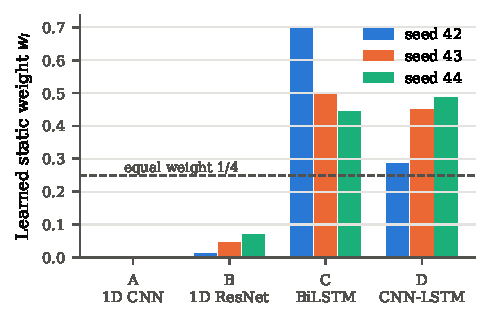
\includegraphics[width=\columnwidth]{weights}
\caption{Static aggregation weights learned on fold 9 for each seed. The dashed line marks the equal
weight 1/4 used by the selected gate.}
\label{fig:weights}
\end{figure}

\subsubsection{Ablation Study on Activation Function and Optimizer}
The choice of activation function and optimizer was examined on Client~D (CNN-LSTM, folds 7--8, seed
42), keeping every other element of the recipe fixed, including the OneCycle schedule with a maximum
learning rate of $10^{-3}$, early stopping on fold 9 and the class-weighted loss. To avoid any tuning
on the test data, the ablations were evaluated on fold 9 only. In the activation ablation the ReLU of
the convolutional blocks and of the classification head was replaced, while the gates of the LSTM were
left unchanged. Tables~\ref{tab:act} and~\ref{tab:opt} report the best fold-9 macro AUROC, the epoch at
which it was reached, the number of epochs before early stopping and the training loss at the selected
epoch.

\begin{table}[!t]
\centering
\caption{Activation-function ablation (Client D, CNN-LSTM, seed 42; fold-9 macro AUROC)}
\label{tab:act}
\footnotesize
\resizebox{\columnwidth}{!}{\begin{tabular}{@{}lccc@{}}
\toprule
Activation & Fold-9 AUROC & Best / run epochs & Train loss \\
\midrule
ReLU (used) & 0.898 & 23 / 31 & 0.444 \\
LeakyReLU & \textbf{0.898} & 24 / 32 & 0.423 \\
ELU & 0.895 & 14 / 22 & 0.547 \\
GELU & 0.896 & 14 / 22 & 0.534 \\
Tanh & 0.894 & 19 / 27 & 0.484 \\
\bottomrule
\end{tabular}
}
\end{table}

\begin{table}[!t]
\centering
\caption{Optimizer ablation (Client D, CNN-LSTM, seed 42; fold-9 macro AUROC; maximum learning rate
$10^{-3}$ for all optimizers)}
\label{tab:opt}
\footnotesize
\resizebox{\columnwidth}{!}{\begin{tabular}{@{}lccc@{}}
\toprule
Optimizer & Fold-9 AUROC & Best / run epochs & Train loss \\
\midrule
AdamW (used) & \textbf{0.898} & 23 / 31 & 0.444 \\
Adam \cite{kingma2015adam} & 0.898 & 20 / 28 & 0.480 \\
SGD (momentum 0.9) & 0.786 & 30 / 38 & 1.014 \\
RMSprop (momentum 0.9) & 0.855 & 3 / 11 & 0.724 \\
\bottomrule
\end{tabular}
}
\end{table}

ReLU and LeakyReLU perform identically (0.898), and they also train longest before early stopping (23
and 24 epochs to the best model), reaching the lowest training losses (0.444 and 0.423). The smooth
activations GELU (0.896) and ELU (0.895) converge faster, with their best epoch at 14, but to a
slightly lower AUROC, and the saturating tanh is the weakest (0.894). The differences are at most 0.004
AUROC, so the activation function is not a decisive design factor for this model, and the ReLU used for
all clients is among the best choices.

The optimizer matters much more. AdamW and Adam reach the same AUROC (0.898), which shows that the
decoupled weight decay neither helped nor hurt at this data size. SGD with momentum is clearly
inferior (0.786): with the same maximum learning rate of $10^{-3}$ it was still improving slowly when
it stopped after 38 epochs, with a training loss of 1.014, so it would need a much larger learning rate
or longer training. RMSprop reached its best AUROC of 0.855 already at epoch 3 and did not improve
afterwards, which indicates unstable optimisation with this learning rate and momentum. Adaptive
moment-based optimizers are therefore the appropriate choice for the clients, and the configuration
used in this work (ReLU with AdamW) is confirmed by both ablations.

% ---------------------------------------------------------------------------------- E
\subsection{Federated Learning Results Analysis}
\label{sec:flresults}

\subsubsection{Client-wise Training Accuracy and Loss}
Because the federation consists of a single round, the training dynamics of the system are those
of the four local trainings. Fig.~\ref{fig:clientcurves} shows, for seed 42, the validation macro
AUROC (the early-stopping criterion, used here in place of accuracy because the label-wise accuracy
depends on thresholds that are fitted only after training) and the weighted training loss of every
client over its local epochs, and Table~\ref{tab:clienttrain} summarises all three seeds.

\begin{figure*}[!t]
\centering
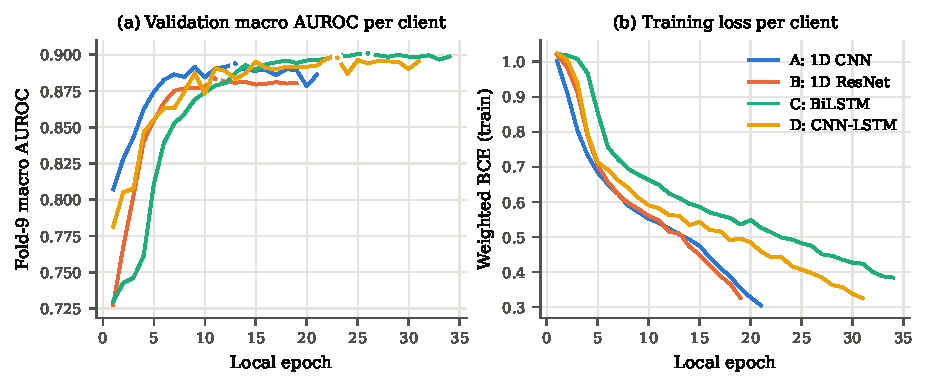
\includegraphics[width=0.9\textwidth]{client_curves}
\caption{Local training of the four clients (seed 42): (a) fold-9 macro AUROC per epoch, with the
selected epoch marked by a dot; (b) class-weighted training BCE per epoch. Each curve ends when early
stopping (patience 8) was triggered.}
\label{fig:clientcurves}
\end{figure*}

\begin{table*}[!t]
\centering
\caption{Client-wise training summary (mean over 3 seeds; loss and AUROC mean $\pm$ SD at the selected epoch)}
\label{tab:clienttrain}
\footnotesize
\begin{tabular}{@{}lcccccc@{}}
\toprule
Model & $n_{\text{train}}$ & Epochs run & Best epoch & Train loss & Fold-9 AUROC & $T_i$ \\
\midrule
Client A & 4{,}277 & 20.7 & 12.7 & 0.510 $\pm$ 0.036 & 0.893 $\pm$ 0.001 & 1.74 $\pm$ 0.22 \\
Client B & 4{,}280 & 21.7 & 13.7 & 0.479 $\pm$ 0.079 & 0.886 $\pm$ 0.002 & 1.52 $\pm$ 0.15 \\
Client C & 4{,}264 & 35.0 & 27.0 & 0.466 $\pm$ 0.017 & 0.900 $\pm$ 0.001 & 1.25 $\pm$ 0.09 \\
Client D & 4{,}263 & 30.7 & 22.7 & 0.450 $\pm$ 0.024 & 0.898 $\pm$ 0.001 & 1.35 $\pm$ 0.06 \\
Pooled (folds 1--8) & 17{,}084 & 31.0 & 23.0 & 0.452 $\pm$ 0.037 & 0.914 $\pm$ 0.002 & 1.31 $\pm$ 0.08 \\
\bottomrule
\end{tabular}

\end{table*}

The convolutional clients converge fastest: Client A reaches its best validation AUROC after 12.7
epochs and Client B after 13.7 epochs on average, after which the validation AUROC stagnates or
decreases while the training loss keeps falling, the typical sign of over-fitting on a small local
dataset. The recurrent clients learn more slowly at the start (Client C stays below 0.80 for the
first four epochs in Fig.~\ref{fig:clientcurves}a) but keep improving for longer, with best epochs
of 27.0 (C) and 22.7 (D), and they end with the highest validation AUROCs (0.900 and 0.898). The
fitted temperatures are all larger than one (1.25--1.74 on average), i.e.\ every client is
over-confident after training with the class-weighted loss, and calibration is therefore needed before
probabilities from different clients can be averaged meaningfully.

\subsubsection{Global Model (Server) Test Accuracy and Loss}
The server performs no iterative training, so there are no communication rounds over which a server
accuracy or loss could converge. The closest analogue is the behaviour of the global model as client
contributions are added. Fig.~\ref{fig:server} plots the macro AUROC of the equal-weight global model
against the number of aggregated clients, both on fold 9 and on the test fold. Both curves rise
monotonically and flatten after three clients: the mean over all subsets increases from 0.890 with
one client to 0.900 with two, 0.903 with three and 0.905 with four on the test fold. The gap between
the fold-9 and the test curves remains small (0.004 for the full federation), which shows that the
validation-based selection did not over-fit the gate. In terms of loss, the selected gate has a
cross-validated binary cross-entropy of 0.372 on fold 9 and a test binary cross-entropy of 0.376
$\pm$ 0.008; the learned static (0.349 $\pm$ 0.004) and dynamic (0.343 $\pm$ 0.005) gates have lower
test losses, mirroring their better calibration on fold 9 (Table~\ref{tab:fusion}), but a lower AUROC.

\begin{figure}[!t]
\centering
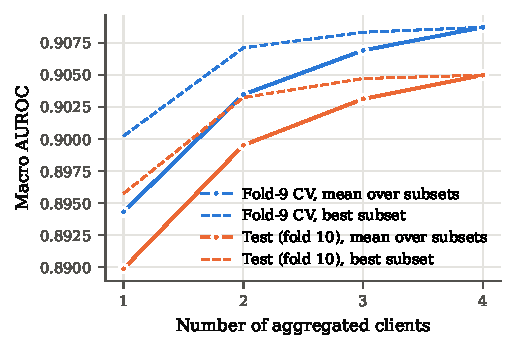
\includegraphics[width=\columnwidth]{server_convergence}
\caption{Macro AUROC of the global (server) model as a function of the number of aggregated clients,
averaged over all subsets of that size (solid) and for the best subset (dashed).}
\label{fig:server}
\end{figure}

\subsubsection{Comparison with Other Federated Learning Frameworks}
Parameter-averaging frameworks cannot combine the heterogeneous clients of CardioSentinel, so they were
evaluated with one shared architecture, the CNN-LSTM of Client~D, on exactly the same four client
partitions. FedAvg \cite{mcmahan2017fedavg}, FedProx \cite{li2020fedprox} ($\mu=0.01$), SCAFFOLD
\cite{karimireddy2020scaffold} (control variates, option II) and FedNova \cite{wang2020fednova}
(updates normalised by the number of local steps) were run for 20 communication rounds of one local
epoch each, with the client recipe of Section~\ref{sec:setup} (AdamW, learning rate $10^{-3}$, batch
128, class-weighted loss, augmentation, gradient clipping) and aggregation weights $n_k/n$. The round
with the best fold-9 macro AUROC was kept, calibrated and thresholded on fold 9, and evaluated once on
the test fold. Because of the computational cost these runs use seed 42 only, so
Table~\ref{tab:fedcomp} reports seed-42 values for every row, and Fig.~\ref{fig:flconv} shows the
convergence.

\begin{table}[!t]
\centering
\caption{Comparison with federated-learning frameworks on the same four client partitions (seed 42;
test fold unless stated). $^{a}$Patient-grouped CV on fold 9.}
\label{tab:fedcomp}
\footnotesize
\setlength{\tabcolsep}{3pt}
\resizebox{\columnwidth}{!}{\begin{tabular}{@{}lcccccc@{}}
\toprule
Method & Rounds & Same arch. & Fold-9 AUROC & Test AUROC & F1 (\%) & Acc. (\%) \\
\midrule
Local only (best client, D) & 0 & -- & 0.898 & 0.895 & 68.9 & 85.0 \\
FedAvg \cite{mcmahan2017fedavg} & 20/20 & yes & 0.911 & 0.907 & 71.8 & 87.2 \\
FedProx ($\mu=0.01$) \cite{li2020fedprox} & 20/20 & yes & 0.910 & 0.906 & 71.4 & 86.9 \\
SCAFFOLD \cite{karimireddy2020scaffold} & 1/20 & yes & 0.850 & 0.842 & 62.4 & 80.6 \\
FedNova \cite{wang2020fednova} & 20/20 & yes & 0.911 & 0.907 & 71.5 & 86.8 \\
\textbf{Proposed (one-shot gate)} & 1 & no & 0.908\textsuperscript{a} & 0.905 & 70.9 & 86.8 \\
\midrule
Centralised (pooled data) & -- & -- & 0.916 & 0.909 & 69.6 & 85.5 \\
\bottomrule
\end{tabular}
}
\end{table}

\begin{figure*}[!t]
\centering
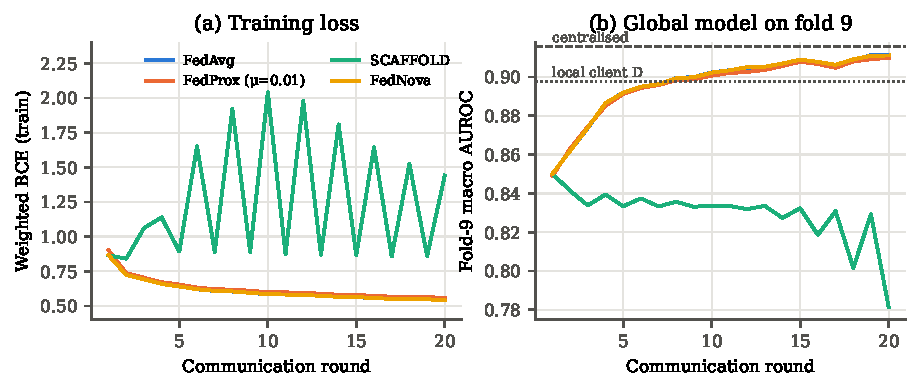
\includegraphics[width=0.9\textwidth]{fl_convergence}
\caption{Convergence of the parameter-averaging frameworks (shared CNN-LSTM, seed 42): (a) training
loss averaged over clients; (b) fold-9 macro AUROC of the global model, with the local-only Client D
and the centrally trained CNN-LSTM as references.}
\label{fig:flconv}
\end{figure*}

\textit{Accuracy.} FedAvg and FedNova reach a test macro AUROC of 0.907 and FedProx 0.906, slightly
above the proposed one-shot gate (0.905) and close to centralised training (0.909). They also achieve a
higher macro F1 (71.4\%--71.8\% versus 70.9\%). With identical clients and many communication rounds,
parameter averaging thus remains marginally more accurate than prediction-level aggregation; the
difference to the proposed model (0.002 AUROC) is, however, smaller than the gain of either approach
over local training (0.895 for Client~D in this seed). SCAFFOLD failed in this configuration: its best
global model was the one after the first round (test AUROC 0.842), and its training loss oscillated
between about 0.8 and 2.0 in subsequent rounds. The control-variate correction assumes plain SGD
local steps of size $\eta$, and combined with the adaptive AdamW updates used here it over-corrects
the client drift; with SGD local training it may behave differently.

\textit{Stability and convergence speed.} FedAvg, FedProx and FedNova converge smoothly and almost
identically (Fig.~\ref{fig:flconv}): they pass the local-only reference of 0.898 on fold 9 at round 8, exceed 0.90 at round 10 and are still improving slightly at round 20, so more rounds could add
a little more. FedNova coincides with FedAvg because all four clients perform the same number of local
steps (33 per epoch), in which case its normalisation has no effect; the proximal term of FedProx is
unnecessary when the label distributions of the clients are as similar as here. The cost of this
accuracy is communication and coordination: 20 synchronised rounds, each exchanging the full set of
0.47M parameters with every client, and the requirement that all institutions train the same network.
The proposed model needs a single round, exchanges only five probabilities per client and query, and
lets every institution keep its own architecture, at a cost of about 0.002 AUROC in this setting.

% ---------------------------------------------------------------------------------- F
\subsection{Class-wise Analysis}
\label{sec:classwise}

\subsubsection{Confusion Matrix}
Fig.~\ref{fig:confusion} shows the per-class confusion matrices of the proposed model on the 2,158
test records for seed 42, at the thresholds chosen on fold 9 (0.42 for NORM, 0.62 for MI and STTC
and 0.64 for CD and HYP), and Fig.~\ref{fig:roc} the corresponding ROC curves. Because the task is
multi-label, each superclass has its own $2\times2$ matrix.

\begin{figure*}[!t]
\centering
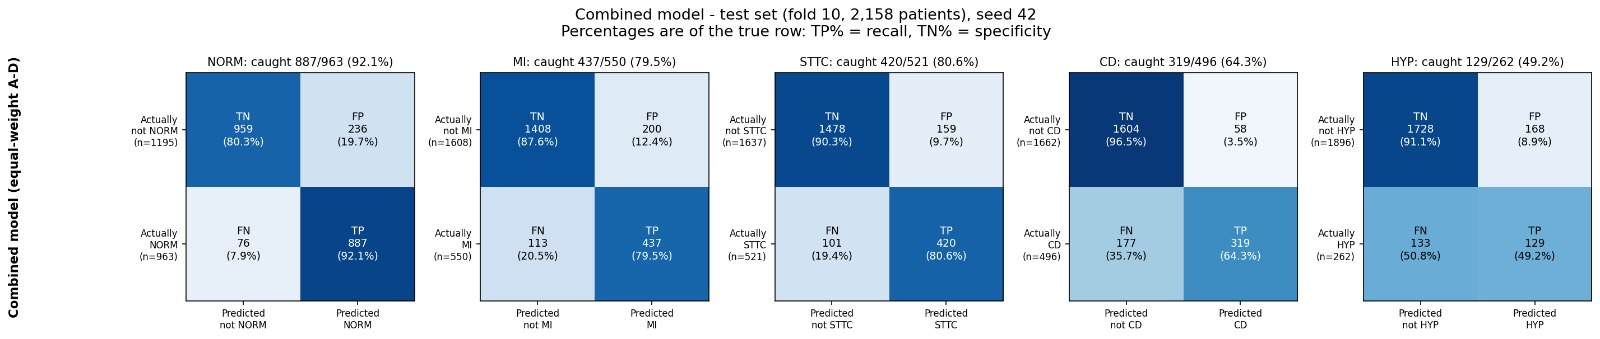
\includegraphics[width=\textwidth]{confusion_combined.jpg}
\caption{Per-class confusion matrices of the proposed model on the test fold (seed 42); counts and
row-normalised rates (TP\% = recall, TN\% = specificity).}
\label{fig:confusion}
\end{figure*}

\begin{figure}[!t]
\centering
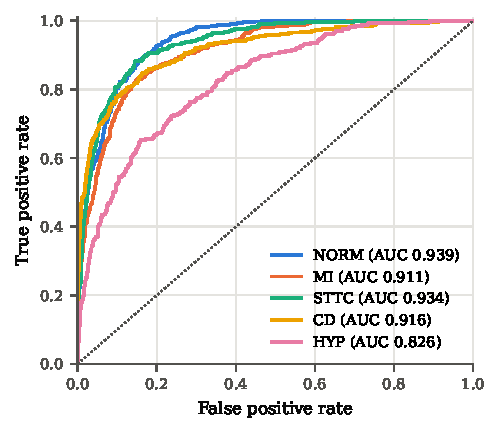
\includegraphics[width=0.9\columnwidth]{roc}
\caption{ROC curves of the proposed model on the test fold for the five superclasses (seed 42).}
\label{fig:roc}
\end{figure}

NORM is detected most reliably: 887 of its 963 positives are found (recall 0.92), at the cost of 236
false positives, which reflects the low NORM threshold that favours sensitivity. For STTC and MI the
model identifies 420 of 521 and 437 of 550 positives, with 159 and 200 false positives respectively.
CD is predicted conservatively: only 58 false positives occur, but 177 of the 496 positives are
missed. HYP is the most difficult class, with 129 true positives, 133 false negatives and 168 false
positives; hypertrophy criteria rely on voltage amplitudes, which the per-recording z-scoring
partly removes, and HYP frequently co-occurs with STTC and CD, so its ECG changes overlap with those
of other classes. The ROC curves confirm this ranking, with the HYP curve clearly below the others.

Compared with the four clients, each at its own fold-9 thresholds (seed 42), for MI the
gate both finds the most positives (437 against 408--431) and raises the fewest false alarms (200
against 226--258). For CD it trades recall for precision: the clients find 314--355 positives with
110--163 false positives, the gate 319 with only 58. The gain of the combination is therefore mainly
in precision, in line with Table~\ref{tab:main}, where the macro precision rises from at most 67.0\%
to 69.8\% while the recall stays at the level of the clients.

\subsubsection{Class-wise Performance Table}
Table~\ref{tab:classwise} reports precision, recall, F1-score and AUROC per superclass, averaged over
the three seeds, together with the macro and support-weighted averages.

\begin{table}[!t]
\centering
\caption{Class-wise performance of the proposed model on the test fold (mean of 3 seeds)}
\label{tab:classwise}
\footnotesize
\setlength{\tabcolsep}{4pt}
\begin{tabular}{@{}lccccc@{}}
\toprule
Class & Precision & Recall & F1-score & AUROC & Support \\
\midrule
NORM & 0.782 & 0.930 & 0.850 & 0.938 & 963 \\
MI & 0.724 & 0.730 & 0.725 & 0.912 & 550 \\
STTC & 0.745 & 0.792 & 0.768 & 0.933 & 521 \\
CD & 0.800 & 0.682 & 0.735 & 0.914 & 496 \\
HYP & 0.439 & 0.490 & 0.461 & 0.828 & 262 \\
\midrule
Macro avg. & 0.698 & 0.725 & 0.707 & 0.905 & 2792 \\
Weighted avg. & 0.735 & 0.780 & 0.753 & 0.917 & 2792 \\
\bottomrule
\end{tabular}

\end{table}

NORM (F1 0.850) and STTC (0.768) are the best-recognised superclasses, followed by CD (0.735) and MI
(0.725). HYP remains clearly weaker (F1 0.461, AUROC 0.828), and because it is also the rarest class
it pulls the macro F1 (0.707) below the support-weighted F1 (0.753). The AUROC of every class except
HYP exceeds 0.91, so the ranking quality is high and the lower F1 values of MI and CD are largely a
matter of operating point.

Fig.~\ref{fig:confusion-mean} gives the confusion matrices averaged over the three seeds. Summed over
the five classes, the model makes 2,177 true-positive and 7,198 true-negative decisions out of 10,790
(2,158 ECGs $\times$ 5 classes), a label-wise accuracy of 0.869 with a micro-averaged precision of
0.731 and recall of 0.780; the 615 false negatives are dominated by HYP (134), CD (158) and MI (148).

\begin{figure*}[!t]
\centering
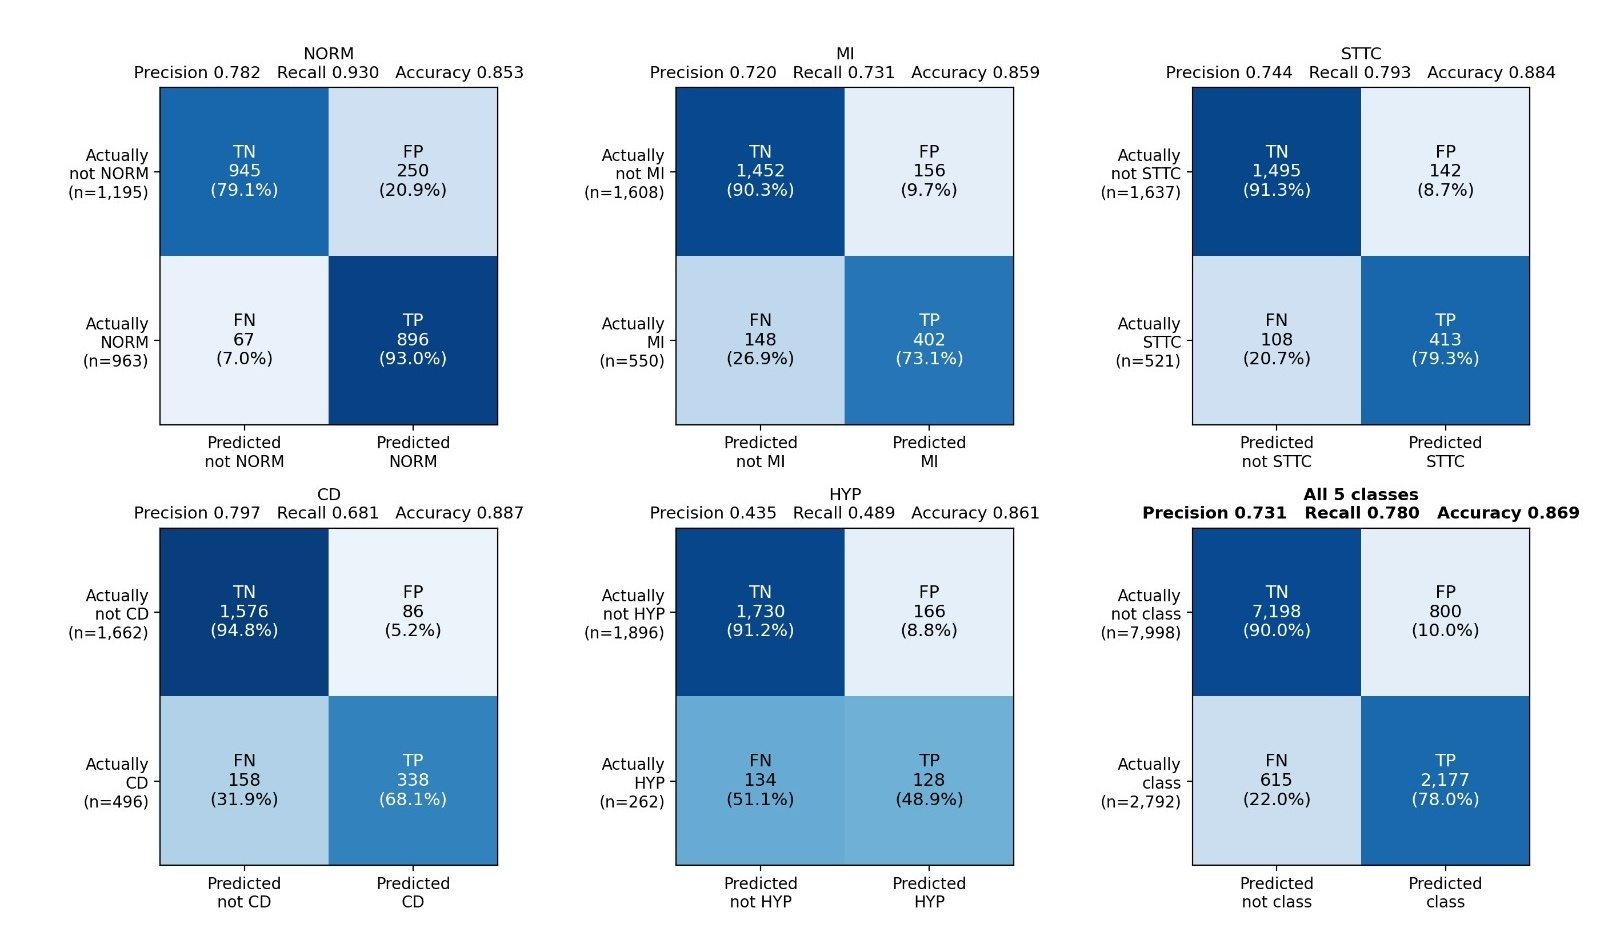
\includegraphics[width=0.85\textwidth]{confusion_mean.jpg}
\caption{Per-class confusion matrices of the proposed model on the test fold (fold 10, 2,158 ECGs), mean
counts over seeds 42, 43 and 44; percentages are of the true row. The last panel sums the five classes
(2,158 ECGs $\times$ 5 decisions = 10,790).}
\label{fig:confusion-mean}
\end{figure*}

\textit{Per-finding triage.} When the clinical requirement is a precision and recall of at least 0.90,
no global threshold can satisfy it for all classes. Applying the rule-in/rule-out bands fitted on
fold 9 (Section~\ref{sec:clf}) to the test fold, 53.7\% of all findings are decided automatically,
with a macro precision of 0.937, a macro recall of 0.908 over the automated classes and an accuracy of
0.967; 17.8\% of the ECGs are decided completely without referral. NORM, MI and CD were automated in
all seeds, STTC in one of three seeds, and HYP only in rule-out mode, so every possible HYP finding is
referred. Not every target was met: the test recall of CD was 0.880.

% ---------------------------------------------------------------------------------- G
\subsection{Explainable Results}
\label{sec:xai-results}

The explanations were computed for the selected equal-weight gate of seed 42 on 300 randomly drawn
validation (fold-9) records, which contain 131 NORM, 81 MI, 65 STTC, 80 CD and 31 HYP positives;
the test fold was not used. Fig.~\ref{fig:xaileads} shows the global lead importance, i.e.\ the share
of the absolute Integrated-Gradients attribution falling on each lead, averaged over the positive
records of each class. Under a uniform distribution every lead would receive 8.3\%.

\begin{figure}[!t]
\centering
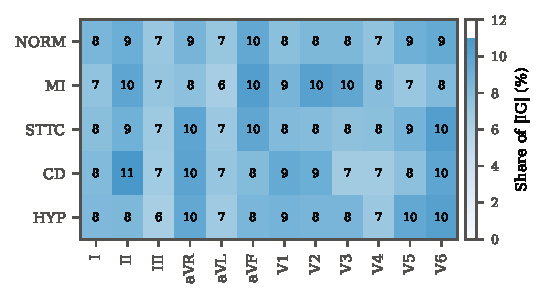
\includegraphics[width=\columnwidth]{xai_leads}
\caption{Global explanation: share of the absolute Integrated-Gradients attribution per lead (\%)
for the positive validation records of each superclass (seed 42, equal-weight gate).}
\label{fig:xaileads}
\end{figure}

The attributions are spread over all twelve leads (no lead receives more than 11.0\%), which is
consistent with the redundancy of the leads shown in Fig.~\ref{fig:leadcorr} and with training under
lead dropout. Within this spread the emphasis follows the expected anatomy. For MI the largest shares
fall on aVF (10.3\%), V2 (10.1\%), II (9.8\%) and V3 (9.7\%), i.e.\ on the inferior and anteroseptal
leads that record the most frequent infarct locations. For HYP the largest shares fall on V6
(10.3\%), V5 and aVR (9.6\% each) and V1 (8.6\%), the leads used by the classical voltage criteria
for left ventricular hypertrophy, which combine the S wave in V1 with the R wave in V5 or V6. For CD
the model relies most on II (11.0\%), aVR (9.9\%), V6 (9.8\%) and V1 (9.4\%); V1 and V6 are the leads
in which right and left bundle branch blocks are recognised. STTC is attributed mainly to the
lateral and inferior leads V6 (10.3\%), aVR (9.8\%) and aVF (9.7\%). In every class, leads III and aVL
are among the four least-attributed leads (6.2\%--7.2\%); both are linear combinations of I and II,
so they add little independent information.

\textit{Local explanations.} Fig.~\ref{fig:xailocal} shows the two validation records predicted with
the highest confidence for MI and for STTC, with the three leads that carry the largest attribution
and the attribution magnitude along time. Record 5927 (label MI) is classified as MI with probability
0.99, and its attribution concentrates on V2, V3 and V4. These leads show deep, predominantly negative
QRS complexes, the pattern of an anterior infarction, and the attribution peaks at each QRS complex
rather than in the baseline between beats. Record 14758 (labels STTC and HYP) receives P(STTC) = 0.98
and P(HYP) = 0.85, so both of its labels are recovered; for STTC the attribution falls on V2, V1 and
aVF and again peaks at the QRS complexes and the adjoining ST segments of the beats. In both cases the
attribution is locked to the beats and falls on the waveform segments a cardiologist would inspect,
not on the baseline between beats; two examples cannot, however, establish this for all records.

\begin{figure*}[!t]
\centering
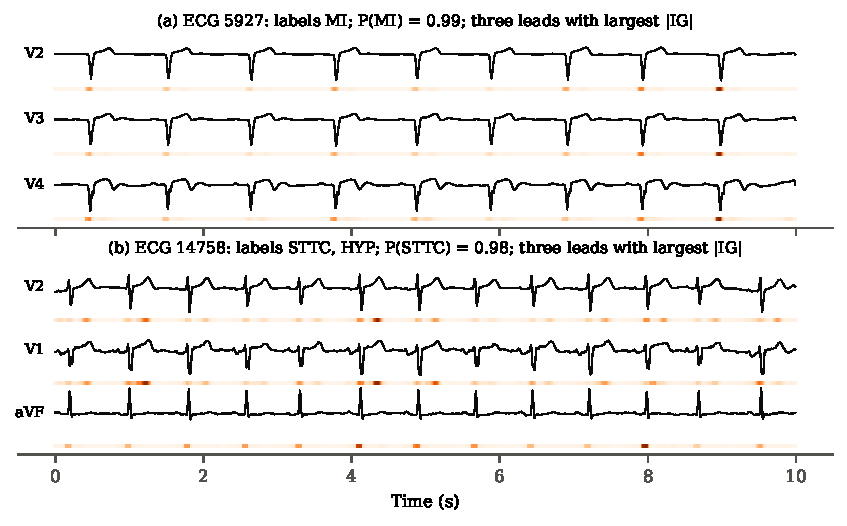
\includegraphics[width=0.95\textwidth]{xai_local}
\caption{Local explanations for the most confident true-positive (a) MI and (b) STTC validation
records. For each record the three leads with the largest total attribution are shown; the colour
strip below each trace encodes $|\mathrm{IG}|$ over time (darker = larger), smoothed over 90~ms.}
\label{fig:xailocal}
\end{figure*}

\textit{Faithfulness.} Table~\ref{tab:deletion} reports the deletion test. For NORM, MI and CD,
removing the lead with the largest attribution lowers the mean predicted probability more than
removing a random lead (NORM: $-$0.028 versus $-$0.019; MI: $-$0.030 versus $-$0.006; CD: $-$0.043
versus $-$0.012), and removing the three most important leads lowers it substantially more than
removing three random leads (NORM: $-$0.135 versus $-$0.074; MI: $-$0.057 versus $-$0.006; CD:
$-$0.070 versus $-$0.009). For these classes the attributions therefore identify leads on which the
prediction actually depends. For STTC and HYP, in contrast, neither targeted nor random deletion
changes the probability appreciably (STTC: 0.764 intact, 0.765--0.772 after deletion; HYP: 0.620
intact, 0.613--0.627 after deletion). The evidence for these two classes is distributed redundantly
over many leads, so lead-level attributions should not be read as identifying a single decisive lead.

\begin{table}[!t]
\centering
\caption{Deletion test: mean gate probability of the true class after zeroing the $k$ leads with the
largest IG attribution or $k$ random leads (fold-9 positives, seed 42)}
\label{tab:deletion}
\footnotesize
\setlength{\tabcolsep}{4pt}
\resizebox{\columnwidth}{!}{\begin{tabular}{@{}lcccccc@{}}
\toprule
 & & & \multicolumn{2}{c}{Top-$k$ IG leads removed} & \multicolumn{2}{c}{Random $k$ leads removed} \\
\cmidrule(lr){4-5}\cmidrule(l){6-7}
Class & $n$ & Mean $p$ (intact) & $k=1$ & $k=3$ & $k=1$ & $k=3$ \\
\midrule
NORM & 131 & 0.741 & 0.713 & 0.606 & 0.722 & 0.667 \\
MI & 81 & 0.750 & 0.720 & 0.693 & 0.744 & 0.744 \\
STTC & 65 & 0.764 & 0.765 & 0.772 & 0.764 & 0.771 \\
CD & 80 & 0.758 & 0.715 & 0.688 & 0.746 & 0.749 \\
HYP & 31 & 0.620 & 0.626 & 0.621 & 0.627 & 0.613 \\
\bottomrule
\end{tabular}
}
\end{table}

\textit{Federation-level explanation.} At the level of the institutions, the Shapley values in
Table~\ref{tab:shapley} show that the four clients contribute comparably to the AUROC of the
federation (0.097--0.105 on the test fold), with the recurrent clients C and D contributing most.
Together with the signal-level attributions, this gives a clinician two complementary views: which
leads and waveform segments drove a finding, and which participating sites the global model relied on.
These explanations are post hoc and were not yet reviewed by cardiologists, and IG with a zero
baseline, like every attribution method, depends on the choice of baseline.


% ---------------------------------------------------------------------------------- H
\subsection{Comparison with State-of-the-Art and Discussion}
\label{sec:discussion}

Table~\ref{tab:sota} compares the proposed model with published results on the PTB-XL superclass
task. The models of \cite{strodthoff2021} were trained centrally on the same folds 1--8 and tested on
the same fold 10, and they are therefore the most directly comparable; the other entries use the
same superclass labels but different training protocols.

\begin{table}[!t]
\centering
\caption{Comparison with state-of-the-art results on the PTB-XL five-superclass task}
\label{tab:sota}
\footnotesize
\setlength{\tabcolsep}{3pt}
\begin{tabular}{@{}p{3.2cm}p{1.6cm}cc@{}}
\toprule
Method & Training data & Macro AUROC & Acc.\ (\%) \\
\midrule
Wavelet + NN \cite{strodthoff2021} & pooled & 0.874 & -- \\
inception1d \cite{strodthoff2021} & pooled & 0.921 & -- \\
LSTM (bidir.) \cite{strodthoff2021} & pooled & 0.921 & -- \\
xresnet1d101 \cite{strodthoff2021} & pooled & 0.928 & -- \\
resnet1d\_wang \cite{strodthoff2021} & pooled & 0.930 & -- \\
Ensemble \cite{strodthoff2021} & pooled & 0.934 & -- \\
ST-MEM \cite{na2024stmem} & pooled + pretrain & 0.933 & 82.5 \\
METS, zero-shot \cite{li2023mets} & pooled + text & -- & 84.2 \\
\midrule
Pooled CNN-LSTM (ours) & pooled & 0.909 & 86.4 (label) \\
XGBoost, 172 features (ours) & pooled & 0.909 & 86.8 (label) \\
FedAvg, CNN-LSTM (ours, seed 42) & 4 sites, 20 rounds & 0.907 & 87.2 (label) \\
\textbf{Proposed (federated)} & 4 sites, 1 round & \textbf{0.905} & \textbf{86.9 (label)} \\
\bottomrule
\end{tabular}
\end{table}

The proposed model does not exceed the best centrally trained models: its macro AUROC of 0.905 is
0.016--0.029 below the centrally trained deep networks and the ensemble of
\cite{strodthoff2021}. Part of
this gap is attributable to the data restriction, since each client sees only 25\% of the training
records, and part to the training recipe, since our own pooled CNN-LSTM reaches 0.909 rather than
0.92--0.93; the recipe (100~Hz input, no test-time augmentation, no external pretraining) was kept
fixed for all models to isolate the effect of federation. The accuracies in Table~\ref{tab:sota} are
not directly comparable either, because ST-MEM and METS report accuracy under their own definitions, whereas the
label-wise accuracy of this work averages the five binary decisions.

\textit{Strengths.} The main strength of the approach is that it delivers most of the benefit of
pooling the data without moving any record or parameter: the federated gate recovers about 70\% of the
AUROC lost by splitting the data and ties the pooled CNN-LSTM in macro F1, with one communication step
and freely chosen architectures. It outperforms every model that can be trained at a single site,
including XGBoost on hand-crafted features (0.898 on average), and comes within 0.002 AUROC of FedAvg,
which needs twenty synchronised rounds and a common architecture. The improvement over the best institution is statistically
significant in every seed, the results are highly reproducible (the SD of the gate's macro AUROC over
seeds is below 0.001), and all modelling choices, including the aggregation rule, were made on
validation data before a single evaluation on the test fold. The triage rule converts the model into a
tool that decides about half of all findings automatically at a precision above 0.93, while stating
explicitly which findings require a cardiologist.

\textit{Limitations.} First, the four clients are simulated partitions of one dataset from one
hospital system with near-identical label distributions, so the benefits of the method under real
inter-site shifts (different devices, populations and label practices) remain to be shown. Second,
fold 9 is used for early stopping, calibration, thresholds and the gate, so validation figures are
optimistic; only the test-fold figures are unbiased. Third, the learned gates did not improve on
equal weighting, which suggests that the per-patient gate lacks informative inputs when all clients
see the same signal. Fourth, HYP remains poorly recognised, and the bootstrap confidence intervals
resample records rather than patients (the test fold contains 2,158 records from 1,877 patients).
Fifth, two baselines are stronger than the proposed model: parameter averaging with a shared
CNN-LSTM (FedAvg and FedNova, 0.907) and, without any federation, XGBoost on hand-crafted features
trained on the pooled data (0.909, macro F1 72.6\%). The latter shows that absolute amplitude features,
which the deep clients do not see, carry information that the current gate cannot exploit; adding a
feature-based client to the federation is an obvious extension. Finally, the federated baselines and the
activation and optimizer ablations were run with a single seed, and the triage and explanation analyses
use seed 42.

\textit{Why federation helps.} The federation helps for two reasons. It enlarges the effective
training set without data sharing: no single client can learn from more than a quarter of the
records, but the gate combines models that together have seen all of them. And because the clients
use different architectures, their errors are only partly correlated, so averaging their calibrated
probabilities reduces variance in the same way as a deep ensemble \cite{lakshminarayanan2017,dietterich2000ensemble}:
every pair of clients already outperforms every single client, even though no client was trained to
complement the others.

\section{Conclusion and Future Work}
\label{sec:conclusion}

This paper presented CardioSentinel, a privacy-preserving, one-shot federated model for the multi-label
classification of 12-lead ECGs into the five PTB-XL diagnostic superclasses. Four clients trained a
1D CNN, a 1D ResNet, a BiLSTM and a CNN-LSTM on disjoint, patient-separated quarters of the training
data, calibrated them, and shared only their class probabilities with a server that combines them on
the probability simplex. A parsimony-first selection on patient-grouped validation predictions chose
equal weighting over learned static weights and a per-patient dynamic gate in all three seeds. On the
untouched test fold the federated model reached a macro AUROC of 0.905 $\pm$ 0.000, a macro F1 of
70.7\% and a label-wise accuracy of 86.9\%, improved on the best single client in every seed
(+0.009 to +0.012 AUROC, paired bootstrap), and came within 0.004 AUROC of a model trained on all
data pooled together while matching its macro F1. It outperformed every model trainable at a single
site, including hand-crafted-feature XGBoost, whereas FedAvg with a shared CNN-LSTM was 0.002 AUROC
better after 20 rounds and pooled-data XGBoost 0.004 better; the proposed scheme therefore trades a small
loss in accuracy for a single communication round and a free choice of architecture. Client-subset ablations and Shapley values showed
that every institution contributes, which is why equal weighting outperformed learned weights that
discard the weaker clients. Integrated Gradients attributed the predictions to leads and waveform
segments, and per-finding triage bands automated 53.7\% of the findings at a precision of 0.937 and an
accuracy of 0.967 while referring the remainder to a cardiologist.

Future work will follow four directions. First, the method will be evaluated on genuinely
heterogeneous institutions with different devices, populations and label distributions, where the
diversity of the clients and the need for a learned gate are expected to be larger. Second, a client
trained on hand-crafted amplitude features, such as the XGBoost model that reached 0.909 AUROC on pooled
data, will be added to the federation, and the parameter-averaging baselines will be repeated over
several seeds and with longer training. Third, the gate will receive inputs that actually differ between
clients, such as additional modalities or site metadata, so that per-patient weighting can become
informative, and formal guarantees such as differential privacy on the shared probabilities will be
studied. Fourth, the recognition of hypertrophy will be improved, for example by restoring absolute
voltage information that per-recording normalisation removes, and the explanations will be validated
with cardiologists.


\bibliographystyle{IEEEtran}
\bibliography{references}

\end{document}
